\documentclass[12pt,twoside,catalan,a4paper]{book}%{amsbook}
\usepackage[T1]{fontenc}
\usepackage[latin1]{inputenc}
\setcounter{secnumdepth}{4}
\setcounter{tocdepth}{4}
\usepackage{amssymb}
\usepackage{amsmath}
\usepackage{amsthm}
\usepackage{graphicx}
\usepackage{algorithmic,algorithm}
\usepackage{glossary}
\makeglossary

\usepackage{subfig}
%\usepackage[intlimits]{amsmath}

\usepackage{listings}
\usepackage{rotating}

\def\versio{Versi\'o 1.0.0\\}%

\makeatletter
%%%%%%%%%%%%%%%%%%%%%%%%%%%%%% Textclass specific LaTeX commands.
 %\numberwithin{section}{chapter}
 %\theoremstyle{plain}    
 \newtheorem{thm}{Teorema}%[section]
 \newtheorem{prop}[thm]{Proposici\'o}
 %\numberwithin{equation}{section}	%% Comment out for sequentially-numbered
 \numberwithin{figure}{section}		%% Comment out for sequentially-numbered
 \usepackage{verbatim}
 %\theoremstyle{plain}
 %\theoremstyle{plain}    
% \newtheorem{algorithm}[thm]{Algorithm} %%Delete [thm] to re-start numbering
 \theoremstyle{definition}   			% Cargar el paquete amsthm.sty
 \newtheorem{defi}{Definici\'o}[chapter]%[section]
% \newtheorem{definition}[thm]{Definici\'o}

\usepackage{babel}
\makeatother

\setcounter{tocdepth}{3}

%%% Abreviaturas

\def\ce{corba e\lgem{}\'{\i}ptica}%
\def\ces{corbes e\lgem{}\'{\i}ptiques}%
\def\CE{Corba E\lgem{}\'{\i}ptica}%
\def\CEs{Corbes E\lgem{}\'{\i}ptiques}%
\def\cf{cos finit}%
\def\cfs{cossos finits}%
\def\Cfs{Cossos finits}%
\def\Cf{Cos finit}%
\def\sgc{subgrup c\'{\i}clic}%
\def\Sgc{Subgrup c\'{\i}clic}%
\def\ecdlp{logaritme discret e\lgem{}\'{\i}ptic}%


%%% Definiciones matem\'aticas especiales

\newcommand{\Z}{\ensuremath{\mathbb{Z}}}%			Enteros
\newcommand{\Q}{\ensuremath{\mathbb{Q}}}%			Racionales
\newcommand{\R}{\ensuremath{\mathbb{R}}}%			Reales
\newcommand{\C}{\ensuremath{\mathbb{C}}}%			Complejos
\newcommand{\A}{\ensuremath{\mathbb{A}_{2}}}%			Plano Af\'{\i}n
\newcommand{\Proy}{\ensuremath{\mathbb{P}_{2}}}%		Plano Proyectivo
\newcommand{\K}{\ensuremath{\mathbb{K}}}%			Cuerpo en general
\newcommand{\F}{\ensuremath{\mathbb{F}}}%			Cuerpo finito en general
\newcommand{\Fp}{\ensuremath{\mathbb{F}_p}}%			Cuerpo finito de orden p (primo)
\newcommand{\EFp}{\ensuremath{E(\mathbb{F}_p)}}%		Curva el\'\{i}ptica sobre un cuerpo finito de orden p (primo)
\newcommand{\EFpbis}{\ensuremath{E/\mathbb{F}_p}}
\newcommand{\Fm}{\ensuremath{\mathbb{F}_{2^m}}}%                Cuerpo finito de caractar\'{\i}stica 2, grado m
\newcommand{\Fq}{\ensuremath{\mathbb{F}_q}}%			Idem id. q (q=p^m, p primo y m entero pos.)
\newcommand{\Zn}[1]{\ensuremath{\mathbb{Z}/#1\mathbb{Z}}}%	Anillo de los enteros mod n
\newcommand{\PaI}{\ensuremath{\mathcal{O}}}%                    Punto en el Infinito
\newcommand{\PaIe}{\ensuremath{\mathcal{O}_{E}}}%               Punto en el Infinito de la curva

%%% Para correciones

\newcommand{\crg}[2]{\fbox{\parbox{\textwidth}{#2}} \begin{quote}\textsc{#1}\end{quote}}

%%%% ``Castellanizaci\'on'' de 'algorithmic.sty'

\renewcommand{\algorithmicrequire}{\textbf{Prerequisit:}}%
\renewcommand{\algorithmicensure}{\textbf{Postrequisit:}}%
\renewcommand{\algorithmiccomment}[1]{/* #1 */}%	
\renewcommand{\algorithmicend}{\textbf{fi}}%
\renewcommand{\algorithmicif}{\textbf{si}}%
\renewcommand{\algorithmicthen}{\textbf{llavors}}%
\renewcommand{\algorithmicelse}{\textbf{si no}}%
\renewcommand{\algorithmicfor}{\textbf{per}}%
\renewcommand{\algorithmicforall}{\textbf{per a tot}}%
\renewcommand{\algorithmicdo}{\textbf{fer}}%
\renewcommand{\algorithmicwhile}{\textbf{mentre}}%
\renewcommand{\algorithmicloop}{\textbf{bucle}}%
\renewcommand{\algorithmicrepeat}{\textbf{repetir}}%
\renewcommand{\algorithmicuntil}{\textbf{fins}}%

\floatname{algorithm}{Algorisme}%

% %%% Teoremas y dem\'as
% \theoremstyle{plain}        			% Cargar el paquete theorem.sty o amsthm.sty
 
% \theoremstyle{definition}   			% Cargar el paquete amsthm.sty
 
 \newtheoremstyle{saltolinea}% name   		% Sacado del 'thmtest.tex'
   {9pt}%               Space above, empty = `usual value'
   {9pt}%               Space below
   {}%                  Body font
   {}%                  Indent amount (empty = no indent, \parindent = para indent)
 %  {\bfseries}%         Thm head font
   {\scshape}%          Thm head font
   {}%                  Punctuation after thm head
   {\newline}%          Space after thm head: \newline = linebreak
   {}%                  Thm head spec
 
 \theoremstyle{saltolinea}   			% Cargar el paquete amsthm.sty
 \newtheorem{algo}{Algorisme}

\begin{document}
\begin{titlepage}

\textsc{\\Escola polit\`ecnica Superior\\Universitat de Lleida\\Enginyeria Inform\`atica}\\


\vfill

\begin{center}

\hrule \vspace{0.4cm}
{ \huge \bfseries Criptografia lliure\\ amb \ces}\\[0.4cm]
 
\hrule \vspace{1.5cm}

% Author and supervisor
\begin{minipage}{0.4\textwidth}
\begin{flushleft} \large
\emph{Author:}\\
Sergi \\\textsc{Blanch i Torn\'e}
\end{flushleft}
\end{minipage}
\begin{minipage}{0.4\textwidth}
\begin{flushright} \large
\emph{Director:} \\
Ramiro \\\textsc{Moreno Chiral}
\end{flushright}
\end{minipage}
 
\vfill
 
% Bottom of the page
{\versio}
{\large Setembre 2008}
 
\end{center}


\end{titlepage}

\newpage
%\maketitle
\tableofcontents{}

%makeindex tfc2c.glo -s tfc2c.ist -t tfc2c.glg -o tfc2c.gls
\glossary{name={PGP},description={Pretty Good Privacy}}
\glossary{name={GnuPG},description={Gnu Privacy Guard}}
\glossary{name={IEEE},description={Institute of Electrical and Electronics Engineers \emph{http://grouper.ieee.org/groups/1363/}}}
\glossary{name={NIST},description={National Institute of Standards and Technology}}
\glossary{name={FIPS},description={Federal Information Processing Standards}}
\glossary{name={RFC},description={Request For Comments}}
\glossary{name={IETF},description={Internet Engineering Task Force}}
\glossary{name={Sage},description={http://www.sagemath.org/}}
\glossary{name={FSF},description={Free Software Foundation \emph{http://www.fsf.org/}}}
\glossary{name={Gnu},description={GNU's Not Unix \emph{http://www.gnu.org}}}
\printglossary

%%%%%%%%%%%%%%%%%%%%%%%%%%%%%%%%%%%%%%%%%%%%%%%%%%%%%%%%%%%%%%%%%%%%%%%%%%%%%%%%%%%%%%%%%%%%%%%%%%%%%%%%%%%%
\chapter*{Agra\"{\i}ments}
%%%%%%%%%%%%%%%%%%%%%%%%%%%%%%%%%%%%%%%%%%%%%%%%%%%%%%%%%%%%%%%%%%%%%%%%%%%%%%%%%%%%%%%%%%%%%%%%%%%%%%%%%%%%

Sempre agra\"{\i}t a en Ramiro per la llibertat donada per al desenvolupament i a l'esfor\c{c} fet per fer-me entendre els conceptes necessaris per despr\'es poder escriure \emph{la} línia de codi i estalviar infinitats de temps en implementaci\'o. El considero un mentor i un gran amic amb qui compartir converses molt m\'es enll\`a de la \ce{}. Realment \'es un referent amb qui es pot parlar absolutament de tot.

Merci tamb\'e als companys Joan Valduvieco, Jordi Llonch i Albert Comerma. Dos d'ells per cedir-me infraestructura de la seva empresa {\tt laigu} on allotjar el \emph{subversion} la web i els pegats per al \emph{GnuPG}. Per\'o molt agra\"{\i}t als tres per aguantar les m\'es pesades explicacions sobre criptografia tot i que no en tinga ni idea.

Gr\`acies al Josep Rodrigo per enredar-me a fer-me pilot d'avionetes aquest \'ultim any. Es un gran des-estressant aquesta activitat.

Merci tamb\'e, als companys de feina del sincrotr\'o, en especial a en Jordi Benach per l'esfor\c{c} al llegir un \emph{draft} i enviar correccions per que aquesta documentaci\'o llueixi millor.

Als pacients de \emph{Cal Curc\'o} (la fam\'{\i}lia) i la meva companya Helena, per l'eterna comprensi\'o mostrada en front la meva dificultat de desconnexi\'o despr\'es una llarga jornada combinant treball i estudi, quan el meu car\`acter no \'es el m\'es amable.

%%%%%%%%%%%%%%%%%%%%%%%%%%%%%%%%%%%%%%%%%%%%%%%%%%%%%%%%%%%%%%%%%%%%%%%%%%%%%%%%%%%%%%%%%%%%%%%%%%%%%%%%%%%%
\chapter{Introducci\'o i objectius}\label{ch:IntroObj}
%%%%%%%%%%%%%%%%%%%%%%%%%%%%%%%%%%%%%%%%%%%%%%%%%%%%%%%%%%%%%%%%%%%%%%%%%%%%%%%%%%%%%%%%%%%%%%%%%%%%%%%%%%%%

Aquest projecte \'es un pas m\'es en l'evoluci\'o d'un projecte major de criptografia de \ce{} en programari lliure. El primer pas es va realitzar quan el curs 2003-2004 \'es va presentar \cite{BM04} com a projecte final de carrera de l'enginyeria t\`ecnica un pegat per al \emph{GnuPG} que ampliava l'oferta criptogr\`afica d'aquest programa lliure cap a les \ces{}. Ja llavors no es volia que la feina s'acabes amb la publicaci\'o de la mem\`oria i prou, i tant l'alumne com el director ten\'{\i}em tota l'intenci\'o de seguir-hi.

Durant el temps que l'estudiant ha realitzat les assignatures corresponets al segon cicle d'inform\`atica, en para\lgem{}el s'ha mantingut una senzilla web\footnote{http://www.calcurco.cat/eccGnuPG/} com a repositori p\'ublic de la feina realitzada. Aix\'{\i} com s'ha anat actualitzant les versions del pegat de \ce{} tamb\'e s'ha afegit documentaci\'o sobre aquestes actualitzacions en forma d'articles que s'han presentat a confer\`encies i congressos per tal de publicitar la feina i reportar que el projecte segueix viu.

Les principals correccions i millores s\'on el que avui compendien aquest projecte en forma de treball final de carrera. S'ha treballat per buscar-hi errors i el p\'ublic escrutini de tenir el codi disponible va donar els seus fruits amb el descobriment per part d'en \emph{Mikael Mylnikov} d'una errada en el procediment de firma digital. Posteriorment es converteix en co\lgem{}aborador al aportar una soluci\'o a la debilitat de l'esquema de xifrat inicialment plantejat que culmina amb l'article \cite{BM06} que justifica el perqu\`e de l'error i el perqu\`e de la soluci\'o proposada.

Tamb\'e posteriorment a aquest criptoan\`alisi \'es va posar de moda una nova perspectiva per atacar els criptosistemes en general. Els anomenats atacs laterals del cap\'{\i}tol \ref{ch:atacsLaterals} s\'on formes de trencar una clau privada trencant una implementaci\'o degut a l'entorn on s'executa. Resulta de gran bellesa t\`ecnica ja que aprofita petits detalls d'enginyeria per resoldre d'una forma molt creativa i econ\`omica el que matem\`aticament resultava impossible i inviable econ\`omicament. Des d'aquest projecte tamb\'e s'han tractat les contramesures des d'un punt de vista tant t\`ecnic sobre la implementaci\'o, com recorrent a recursos matem\`atics per invalidar alguns d'aquests intents laterals de criptoan\`alisi.

Una avantatge molt important de les \ces{} que no es explotada per les implementacions en general s'est\`a intentant resoldre des d'aqu\'{\i}. El setup dels criptosistemes e\lgem{}\'{\i}ptics, d'ara endavant  \emph{ECC}s, sempre son preestablerts per a l'usuari i se li donen \ces{} base amb les que fer criptografia. Aix\`o fa que la gran avantatge de canviar de corba per un usuari el deixi obligat a la mateix soluci\'o que en el cas dels \cfs{} amb l'augment de la longitud de la seva clau. En el cap\'{\i}tol \ref{ch:EstrellesIso} es busca de treballar amb conjunts de \ces{} per buscar que l'usuari final tingui la possibilitat de canviar de \ce{} sense tenir que renunciar a una longitud que consideri adequada. Com s'explicar\`a amb detall en el corresponent cap\'{\i}tol, encara no hi ha una implementaci\'o en el projecte que es dongui com a bona per a us p\'ublic.

Finalment, un punt d'inflexi\'o en aquest projecte \'es la inclusi\'o directa dins de la rama de desenvolupament de la llibreria matem\`atica \emph{libgcrypt} del \emph{GnuPG} i la signatura d'una \emph{assigment} amb la \emph{Free Software fundation} (FSF) per la participaci\'o directa i activa en el projecte \emph{Gnu}. Amb aquesta signatura es fa un pas de gegant per permetre aquest projecte existir dins del software lliure amb independ\`encia. Totes dues parts guanyem amb aquesta uni\'o, facilitant l'acc\`es i el desenvolupament; i tamb\'e conseguint suport per a \ces{} en aquest software mundialment ext\`es.

% \begin{enumerate}
%  \item historieta del PGP
%  \item hist\'oria del GnuPG
%  \item origen i evoluci\'o del projecte eccGnuPG (el passat del projecte, el tfc de la t\`ecnica)
%  \item compendiar el treball fet despr\'es de \cite{BM04} (libgcrypt)
%  \begin{enumerate}
%   \item el treball fet per protegir dels atacs laterals
%   \item el treball iniciat amb les isog\`enies (reseteig del setup amb estrelles de \ce)
%   \item assignment amb la \emph{FSF} per la integraci\'o al \emph{GnuPG}
%  \end{enumerate}
% \end{enumerate}

%%%%%%%%%%%%%%%%%%%%%%%%%%%%%%%%%%%%%%%%%%%%%%%%%%%%%%%%%%%%%%%%%%%%%%%%%%%%%%%%%%%%%%%%%%%%%%%%%%%%%%%%%%%%
\chapter{Criptologia de \ce}\label{ch:criptologiaEC}
%%%%%%%%%%%%%%%%%%%%%%%%%%%%%%%%%%%%%%%%%%%%%%%%%%%%%%%%%%%%%%%%%%%%%%%%%%%%%%%%%%%%%%%%%%%%%%%%%%%%%%%%%%%%

Abans de poder entrar a l'algor\'{\i}smica de les \ces{} s'han de prefilar una introducci\'o a l'aritm\`etica d'aquestes. Com a convenci\'o s'ha utilitzat una notaci\'o tipus a la apareguda en la normativa \cite{P1363} que ser\`a aprofundida en la secci\'o \ref{subsec:normes} junt amb altres normatives que influeixen les implementacions de \ce{}.

%%%%%%%%%%%%%%%%%%%%%%%%%%%%%%%%%%%%%%%%%%%%%%%%%%%%%%%%%%%%%%%%%%%%%%%%%%%%%%%%%%%%%%%%%%%%%%%%%%%%%%%%%%%%
\section{Aritm\`etica de \ce}\label{sec:aritmEC}
%%%%%%%%%%%%%%%%%%%%%%%%%%%%%%%%%%%%%%%%%%%%%%%%%%%%%%%%%%%%%%%%%%%%%%%%%%%%%%%%%%%%%%%%%%%%%%%%%%%%%%%%%%%%

Tota la base necess\`aria per comprendre i treballar amb les \ces{} \'es l'algebra. Comen\c{c}ant des del principi es donen alguns conceptes per coneguts i es parteix de la definici\'o de group o conjunt amb una llei de composici\'o interna.

\begin{defi}\label{def:group}
Donat un conjunt $G$ i una llei de composici\'o interna $\oplus$, anomenem grup $\left(G,\oplus\right)$ si compleix:
\begin{enumerate}
 \item $\forall x,y,z \in G, \oplus$ \'es associativa: $\left(x\oplus y\right) \oplus z = x\oplus \left( y \oplus x \right)$.
 \item $\exists e_0 \in G: \forall x \in G$ tal que $x \oplus e_0 = e_0 \oplus x = x$.
 \item $\forall x \in G, \exists y \in G$ que \'es l'invers tal que $x \oplus y = y \oplus x = e_0$.
\end{enumerate}
A m\'es, nomenem a un grup \emph{Abeli\`a} quan a m\'es de les propietats anteriors, l'operaci\'o es commutativa.
\end{defi}

L'estructura sobre la que es realitza l'aritm\`etica de \ces{} \'es un grup. Ampliant la primera operaci\'o que pot tenir un grup, podem donar-li una segona llei de composici\'o interna de manera que formi un anell.

\begin{defi}\label{def:ring}
Donat un conjunt $A$ i dues lleis de composici\'o interna $\oplus$ i $\otimes$, anomenem anell a $(A,\oplus,\otimes)$ si compleix:
\begin{enumerate}
 \item $\left(A,\oplus\right)$ \'es un grup Abeli\`a.
 \item $\exists e_1 \in A,\; e_1\ne e_0: \forall x \in G$ tal que $x \otimes e_1 = e_1 \otimes x = x$.
 \item $\forall x,y,z \in G $ l'operaci\'o $\otimes$ \'es distributiva respecte a $\oplus$: $x \otimes \left( y \oplus z \right) = \left(x \otimes y \right) \oplus \left( x \otimes z \right)$.
\end{enumerate}
\end{defi}
L'exemple cl\`assic d'anell \'es el nombre enters, $\left(\Z,+,\cdot\right)$. Resulta evident es seg\"uent resultat:
\begin{prop}
 S\'{\i} $\left( \mathbb{A},\oplus,\otimes \right)$ \'es un anell, el conjunt $\mathbb{A}^*$ dels seus elements invertibles \'es un grup amb $\otimes$.
\end{prop}
A partir d'aqu\'{\i} la definici\'o de \emph{cos} \'es natural:
\begin{defi}
 Definim un cos $\K$ com un anell on cada element no nul es invertible, es a dir $\K^*=\K\setminus\{e_0\}$.
\end{defi}
L'estructura algebr\`aica sobre la que definirem el grup de punts d'una \ce{} \'es un cos. Tenim molts cossos en la nostra aritm\`etica. Per exemple, amb dues operacions com la suma i el producte, tenim els nombres racionals, $\Q$, els reals, $\R$ o els complexes, $\C$. De manera general un cos amb dues operacions el denotem $\left(\K,\oplus,\otimes\right)$.


%%%%%%%%%%%%%%%%%%%%%%%%%%%%%%%%%%%%%%%%%%%%%%%%%%%%%%%%%%%%%%%%%%%%%%%%%%%%%%%%%%%%%%%%%%%%%%%%%%%%%%%%%%%%
\subsection{\Cfs{}}\label{sec:cfs}

Un cop tenim l'algebra b\`asica definida podem acurar m\'es el seu entorn i afegir restriccions per obtenir les propietats que necessitem. Entrarem aix\'{\i} a l'aritm\`etica modular amb la definici\'o dels \emph{\cfs} o \emph{cossos de Galois}.

\begin{defi}\label{def:finiteField} Un \cf{} \'es un cos amb un nombre finit d'elements.\end{defi}

Al nombre d'aquests elements l'anomenarem \emph{ordre} del cos. Denotarem els \cfs{} com $\F$ o be $\Fq$, si es vol deixar pal\'es el seu ordre, $\left|\Fq\right|=q$. S'obt\'e el seg\"uent resultat fonamental,
\begin{thm}  Per tot primer $p$ i qualsevol $r\in\mathbb{Z}_{>0}$ existeix un \cf{} amb $q = p^r$ elements. Aquest cos \'es \'unic i es denota com \Fq. Reciprocament, si $\Fp$ \'es un \cf{} es t\'e que $\left|\F\right|=q=p^r$, on $p$ \'es un enter primer, anomenat \emph{caracter\'{\i}stica}, i $r\in\mathbb{Z}_{>0}$, conegut com \emph{extensi\'o} o \emph{\'{\i}ndex de l'extenci\'o}.\end{thm}

En endavant usarem \cfs{} en els que l'extensi\'o es $r=1$, per tant es tracta de cossos d'ordre primer, $q=p$: s\'on els \cfs{} \emph{primers}. L'aritm\`etica en aquests cossos \'es l'aritm\`etica m\'odul $p$, i.e., $\Fp$ es pot identificar com $\mathbb{Z}/p\mathbb{Z}$. La criptografia de clau p\'ublica cl\`assica ha usat aquest cossos primers, m\'es precisament el grup multiplicatiu $\Fp^*$, en els criptosistemes basats en el problema anomenat del \emph{logaritme discret}. I la criptografia amb \ces{} torna a usar-los en el basats en el \emph{\ecdlp{}}: ara el grup es troba constitu\"{\i}t pel conjunt de punts de la \ce{} \emph{definida sobre $\Fp$}.


%%%%%%%%%%%%%%%%%%%%%%%%%%%%%%%%%%%%%%%%%%%%%%%%%%%%%%%%%%%%%%%%%%%%%%%%%%%%%%%%%%%%%%%%%%%%%%%%%%%%%%%%%%%%
\subsection{Plans afins i projectius}\label{sec:plans}
Abans d'entrar a definir les \ces{} es fa un rep\`as sobre geometria en el pla, en especial perqu\`e servir\`a per entrar a definir uns plans m\'es interessant per a la \ce{}. Cl\`assicament, quan parlem de plans pensem en dues dimensions on cada punt pot ser definit per un parell ordenat d'elements d'un conjunt. M\'es concretament per situar un punt sobre un pla real utilitzariem un parell ordenat de valors reals, $(x,y)\in\mathbb{R}\times\mathbb{R}$. Per\`o hi ha altres tipus de plans com s\'on els plans projectius que utilitzen una terna ordenada d'elements del conjunt per definir un punt bidimensional.

\begin{defi}\label{def:coorproj}
Donat un cos $\F$ el \emph{pla projectiu} sobre $\F$, $\Proy(\F)$, es defineix com el quocient
$$\Proy(\F)=\frac{\F^3\setminus\left\{(0,0,0)\right\}}{\sim},$$
on $\sim$ \'es la relaci\'o d'equival\`encia definida en $\F^3\setminus\left\{(0,0,0)\right\}$ com $(x,y,z)\sim (x',y',z')$ si existeix $\lambda\in\F^*$, tal que $x=\lambda x', y=\lambda y', z=\lambda z'$.
\end{defi}
Un punt projectiu \'es denota com $[X:Y:Z]\in\Proy(\F)$. La recta $Z=0$ s'anomena \emph{recta en l'infinit}. Es pot fer una aplicaci\'o entre els punts del pla af\'{\i}, $\mathbb{A}_{2}(\F)=\F^{2}$, i els del  pla projectiu $\Proy(\F)$,
$$\begin{array}{rcl}f:\,\mathbb{A}_{2}(\F) & \longrightarrow & \Proy(\F)\\ (x,y) & \longmapsto & \left[x:y:1\right].\end{array}$$
Per\`o la rec\'{\i}proca no \'es una aplicaci\'o ja que resulta evident que la recta projectiva en l'infinit to t\'e representaci\'o en el pla af\'{\i},
$$\begin{array}{rcl}f_{-1}:\,\Proy(\F) & \longrightarrow & \mathbb{A}_{2}(\F)\\ \left[X:Y:Z\right] & \longmapsto & \begin{cases}\left(\frac{X}{Z},\frac{Y}{Z}\right), & \text{si }Z\ne 0,\\ \nexists, & \text{si }Z=0.\end{cases}\end{array}$$


%%%%%%%%%%%%%%%%%%%%%%%%%%%%%%%%%%%%%%%%%%%%%%%%%%%%%%%%%%%%%%%%%%%%%%%%%%%%%%%%%%%%%%%%%%%%%%%%%%%%%%%%%%%%
\subsection{Definint \ces}\label{subsec:def_ces}

Ja tenim tot el necessari sobre \cfs{} aix\'{\i} com tamb\'e sobre plans projectius i ara ens podem posar a \emph{dibuixar} corbes per aquest pla com a subconjunts dels elements d'aquests plans que compleixen una regla particular:

%\begin{defi}\label{def:ce}  Anomenem \ce{} a tota corba {\bf no} singular i absolutament irreductible definida sobre \K{} de genere $1$ amb, com a m\'{\i}nim un punt $K$-racional. Una corba no singular es aquella que compleix,
%\begin{equation} \Delta=-\left(4a^{3}+27b^{2}\right)\neq 0\end{equation}
%\end{defi}

%Una \ce{} compleix una equaci\'o on donada la coordenada en $x$ del parell ordenat af\'{\i} es pugui extreure el resultat com una aplicaci\'o.

\begin{defi} Una \ce{} \EFpbis{} est\`a definida en $\mathbb{P}_{2}(\Fp)$, per una equaci\'o en la \emph{forma normal de Weierstra\ss{} (Weierstra\ss{} Normal Form, WNF)},
\begin{eqnarray}\label{eq:WNF} \lefteqn{F(X,Y,Z)=}\nonumber\\ & & Y^{2}Z+a_{1}XYZ+a_{3}YZ^{2}-X^{3}-a_{2}X^{2}Z-a_{4}XZ^{2}-a_{6}Z^{3}=0,\end{eqnarray}
amb coeficients $a_i\in\Fp$ i sense punts singulars, que vol dir que no res\'ol el seg\"uent sistema d'equacions:
$$\left.\begin{array}{c} \frac{\partial F\left(X,Y,Z\right)}{\partial X}=0\\ \frac{\partial F\left(X,Y,Z\right)}{\partial Y}=0\\ \frac{\partial F\left(X,Y,Z\right)}{\partial Z}=0\\ F\left(X,Y,Z\right)=0\end{array}\right\}$$
\end{defi}

Hi ha reduccions de l'equaci\'o WNF, com per exemple la que hem utilitzat principalment en aquest projecte,

\begin{defi} Per \cf{} de caracter\'{\i}stica diferent de $2$ i $3$, l'equaci\'o \ref{eq:WNF} pot substituir-se per la \emph{forma redu\"{\i}da de Weierstra\ss{} (WRF)},
\begin{equation}\label{eq:WRF} Y^{2}Z=X^{3}+aXZ^{2}+bZ^{3},\end{equation}
i es pot tradu\"{\i}r a un pla af\'{\i},
\begin{equation} \frac{Y^{2}}{Z^{2}}=\frac{X^{3}}{Z^{3}}+a\frac{X}{Z}+b,\ \boxed{\begin{array}{ccc}\frac{Y}{Z} & \rightarrow & y\\ \frac{X}{Z} & \rightarrow & z\end{array}}\Rightarrow y^{2}=x^{3}+ax+b.\end{equation}
\end{defi}
La condici\'o de no--singularitat \'es equivalent a la de no anulaci\'o del discriminant, que en la WRF se pot escriure,
\begin{equation} \Delta=-\left(4a^{3}+27b^{2}\right)\neq 0.\end{equation}

Donada l'equaci\'o de la \ce{} \'es moment de definir el conjunt de punts $E(\Fp)$, ja que ser\`a amb aquest conjunt amb el que depr\'es voldrem fer criptografia.
\begin{defi}\label{def:EFp} El conjunt de punts de una \ce{} $E/\Fp:\;y^2=x^3+ax+b$, que denotem \EFp, \'es el conjunt de punts del pla que compleixen amb l'equaci\'o de la corba, juntament amb el punt en l'infinit, en el pla af\'{\i}, \A,
\begin{equation} \EFp=\left\{ (x,y)\in\Fp^2:\;y^{2}=x^{3}+ax+b\right\} \cup\left\{ \mathcal{{O}}_{E}\right\}.\end{equation}
I en el pla projectiu, \Proy,
\begin{equation} \EFp=\left\{[X:Y:Z]\in\Proy(\Fp):Y^{2}Z=X^{3}+aXZ^{2}+bZ^{3}\right\}.\end{equation}
\end{defi}

%%%%%%%%%%%%%%%%%%%%%%%%%%%%%%%%%%%%%%%%%%%%%%%%%%%%%%%%%%%%%%%%%%%%%%%%%%%%%%%%%%%%%%%%%%%%%%%%%%%%%%%%%%%%
\subsection{Grup de punts}\label{subsec:addMulPunts}

Definides les \ces{} ja podem entrar a veure que podem fer amb elles. D'una forma gen\`erica primer, i entrant en l'us criptogr\`afic despr\'es. Per visualitzar les operacions entre punts d'una \ce, el m\'es efica\c{c} \'es veuren la seva representaci\'o gr\`afica en el pla real $\R^2$.
\begin{defi}\label{def:sumaEracional} Donats dos punts racionals $P\ne Q$ d'una \ce{} $E$, la l\'{\i}nia recta que passa per ambdos ha de intersecar la \ce{} per un tercer punt racional, l'oposat del qual es la suma $P+Q$.\end{defi}
En la figura \ref{fig:sumaEracional} es pot veure un exemple gr\`afic de com seria una suma de dos punts d'una \ce.

\begin{figure}[ht]
\centering
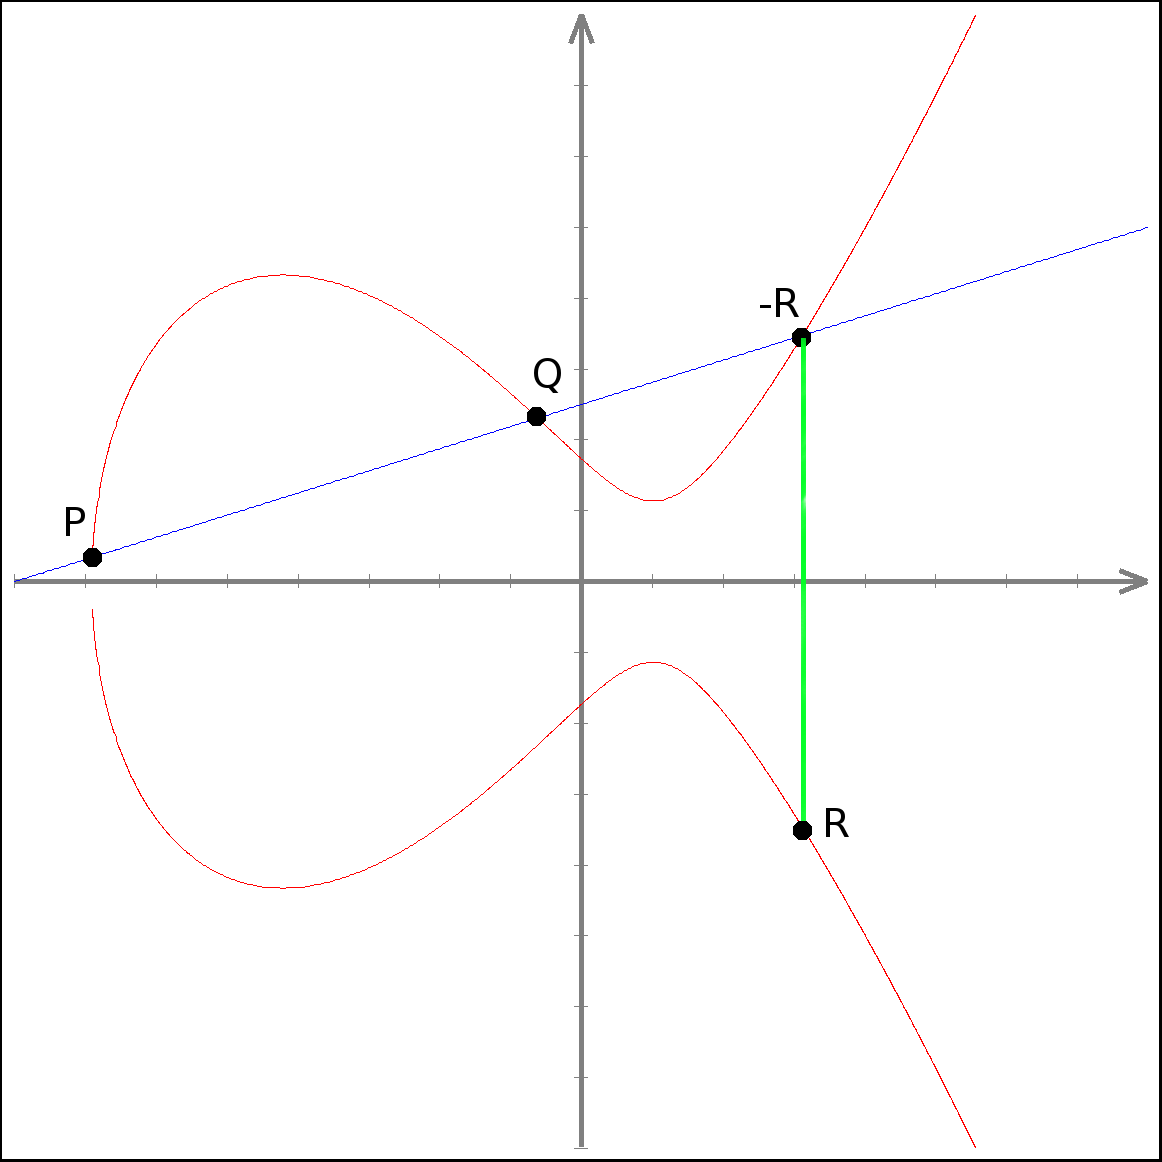
\includegraphics[width=0.5\textwidth]{plots/curve1_mod.png}
\caption{Suma de punts d'una \ce \label{fig:sumaEracional}}
\end{figure}

\begin{defi}\label{def:duplEracional} Donat un punt racional $P$ d'una \ce{} $E$, la l\'{\i}nia recta tangent a aquell punt de la corba interseca la \ce{} per un segon punt racional, l'invers del qual es la suma del punt $P$ amb si mateix, $[2]P=P+P$. Si la tangent resulta ser una recta vertical, la intersecci\'o \'es amb el \emph{punt en l'infinit}, \PaI, que tamb\'e pertany a la corba per\`o no te representaci\'o sobre el pla af\'{\i}: es diu que $P$ \'es d'ordre $2$ ja que $[2]P=\mathcal{O}$.
\end{defi}
En la figura \ref{fig:duplEracional} es pot veure un exemple gr\`afic de com seria un doblat d'un punt d'un \ce.

\begin{figure}[ht]
\centering
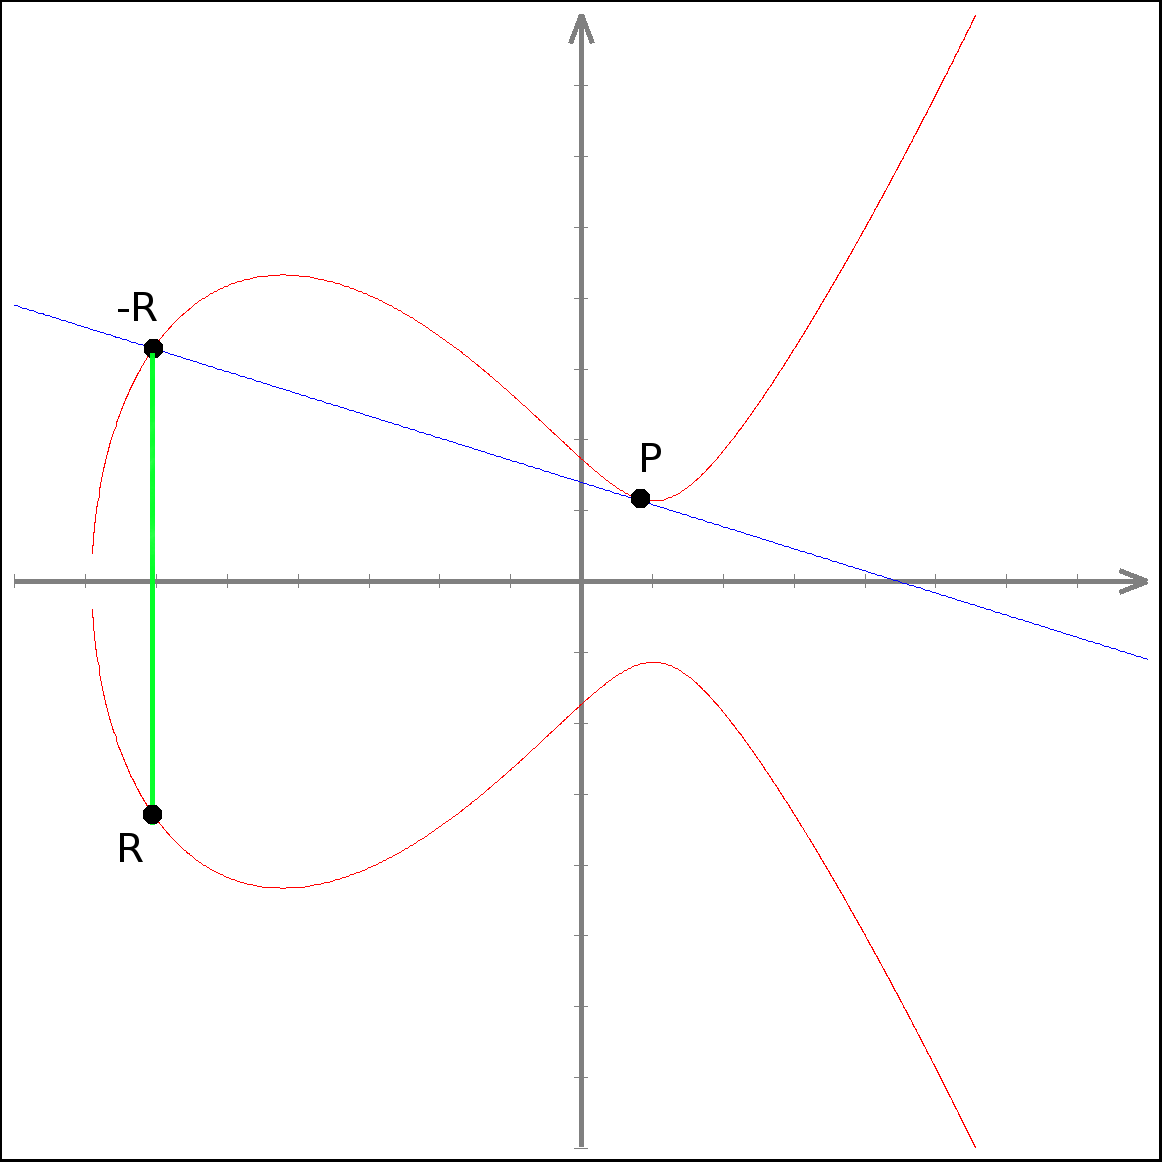
\includegraphics[width=0.5\textwidth]{plots/curve2_mod.png}
\caption{Duplicat d'un punt d'una \ce \label{fig:duplEracional}}
\end{figure}

Existeix, per suposat, una formulaci\'o anal\'{\i}ica d'aquesta suma en $E(\Fp)$, les equacions de la qual, que son les que s'implementen, \'es poden veure per exemple en \cite{HANDECC,LMS265}.
\begin{prop}\label{prop:grpunts} El conjunt de punts d'una \ce{} amb aquesta suma, $\left(E(\Fp),+\right)$, \'es un grup abeli\`a on el neutre \'es el punt en l'infinit, $\mathcal{O}_E$.\end{prop}

L'\emph{ordre} del  grup de punts de $E(\Fp)$ o ``cardinal de la \ce{}'', que denotem com $\left|E(\Fp)\right|$, \'es una data que s'ha de saber per a la posada en funcionament, o \emph{setup}, de un ECC. El seu c\`alcul \'es fa mitjan\c{c}ant l'algorisme SAE, per\`o per la seva complexitat resulta freq\"u\`ent (\cite{NIST186}) que sigui una dada que acompanyi als coeficients i la resta de dades necess\`aries per definir la \ce{}. De tota manera, el \emph{teorema de Hasse} ens acota sempre aquest valor del cardinal de la corba.

\begin{thm}[Hasse]\label{teo:hasse} Donada una \ce{} $E/\Fq$, es compleix que
\begin{equation}\label{eq:hasse} q+1-2\sqrt{q}\le \left|E(\Fq)\right|\le q+1+2\sqrt{q}.\end{equation}
\end{thm}
Aquest teorema permet un enunciat alternatiu usant el par\`ametre $t$, \emph{tra\c{c}a del endomorfisme de Forbenius}: $\left|E(\Fq)\right|=q+1-t$, on $\left|t\right|\le 2\sqrt{q}$. Aqu\'{\i} es veu clar que $\left|E(\Fq)\right|\approx q$, es a dir, l'ordre del grup de punts de la corba \'es aproximadament l'ordre del \cf{} sobre el que est\`a definida.

Donades del definicions \ref{def:sumaEracional} i \ref{def:duplEracional} podem deduir que al punt racional resultant d'un doblat li podem tornar a sumar el mateix. Ens anir\`a be tenir una operaci\'o \emph{suma repetida}.

\begin{defi}\label{def:multEracional} Donat $n\in\Z$ i un punt $P$ d'una \ce{} $E$, anomenem \emph{producte per un escalar} a la suma del punt $P$ amb si mateix un nombre $n$ de vegades,
$$[n]P=\begin{cases}\overbrace{P+\cdots+P}^{n)}, &\text{si }n>0,\\ \mathcal{O}, &\text{si }n=0,\\ \overbrace{(-P)+\cdots+(-P)}^{n)}, &\text{si }n<0.\end{cases}$$
\end{defi}

\'Es amb aquesta operaci\'o \emph{producte d'un punt per un escalar} sobre la que tot gira. M\'es endavant, a partir de la definici\'o \ref{def:ciclic}, veurem com pren forma el criptosistema en base aquesta definici\'o \ref{def:multEracional}.

% \subsubsection{Compressi\'o de punts}
% 
% Les \ces tenen una gran aplicaci\'o, degut a la seva menor longitud i la possibilitat de reseteig, en sistemes amb restriccions de cpu, de mem\`oria i/o d'ample de banda. Tot i aix\`o la difer\`encia no acaba de ser directa, ja que quan sobre un criptosistema definit sobre enters modulars transmetem valors d'una longitud similar al m\`odul, diguem-n'hi $n$; en \ces tenim que transmetre valors menors per\`o al ser punts hem de transmetre coordenades.
% 
% Sobre una \EFp, definida sobre un \cf arbitrari \Fp, un punt estar\`a composat de dues coordenades afins (\A), t\'{\i}pus $(P_x,P_y)$ o incl\'us tres de projectives (\Proy), t\'{\i}pus $[P_X:P_Y:P_Z]$, on cada coordenada t\'e una longitud $p$ de manera que transmetriem $\left(2\cdot p\right)$ o incl\'us $\left(3\cdot p\right)$ en el cas de coordenades projectives.
% 
% Una soluci\'o possible a aquesta situaci\'o passa per reduir un punt a una coordenada af\'{\i} en $x$ i especificar amb un sol bit el signe de la soluci\'o a l'equaci\'o de la \ce.
% 
% S'ha d'anar amb precauc\'o amb aquest recurs, ja que penalitzar\`a en un de cpu a emisor i receptor de la clau p\'ublica a la vegada que minimitzar\`a la transmissi\'o pel canal.
% 
% Les especificacions i est\`andards en fan refer\`encia, tot i que en general es treballa amb punts no comprimits ja que segueixen essent menors que els equivalents sobre \cfs. De tota manera, correm amb la lacra que \emph{certicom} (empresa canadenca lider en \ces) mant\'e patents sobre la compressi\'o de punts entre molts altres algorismes per \ces{}.

%%%%%%%%%%%%%%%%%%%%%%%%%%%%%%%%%%%%%%%%%%%%%%%%%%%%%%%%%%%%%%%%%%%%%%%%%%%%%%%%%%%%%%%%%%%%%%%%%%%%%%%%%%%%
\subsection{Logaritme discret e\lgem{}\'{\i}ptic}

Definides les operacions que podem realitzar amb les \ces{} anem a entrar en la criptografia. Per poder fer criptografia de \ce{} necessitem el mateix que es fa anar quan es planteja sobre \cfs{}:  all\'{\i} s'usa el grup multiplicatiu del cos, $\left(\Fp^*,\cdot\right)$, que \'es sempre un grup c\'{\i}clic d'ordre $p-1$; amb \ces{} tindrem tamb\'e un \sgc{} del grup de punts de la \ce{} i sobre aquest es planteja el \ecdlp{}.

\begin{defi}\label{def:ciclic} Definim un \emph{subgrup c\'{\i}clic} d'una \ce{} com el conjunt de punts generat per un $G\in E(\Fp)$,
\begin{equation}\left\langle G\right\rangle = \left\{ G,[2]G,[3]G,\ldots,[n]G=\mathcal{O}_{E} \right\},\end{equation}
on $n$ \'es l'ordre d'aquest subgrup c\'{\i}clic, 
$$n=\mathrm{ord}(G)=\min\left\{r\in\Z_{>0}:\;[r]G=\mathcal{O}_{E}\right\}.$$
\end{defi}
Per ``aprofitar'' els bits que es disposa \'es necessita un ordre $n$ gran, $n\approx p$, degut a que, como s'ha dit m\'es amunt, $\left|E(\Fp)\right|\approx p$. Pel \emph{teorema de Lagrange} sabem que $\mathrm{ord}(G)\mid\left|E(\Fp)\right|$, es a dir, que l'orden del \sgc{} sobre el que es planteja el criptosistema divideix a l'orden de tot el grup de punts.
\begin{defi}\label{def:cofactor} \'Es defineix el \emph{cofactor} com la relaci\'o entre el cardinal de la \ce{} i l'ordre que t\'e aquest subgrup,
\begin{equation}h=\frac{\left|E(\Fp)\right|}{n}.\end{equation}
\end{defi}

Recordant l'operaci\'o \emph{producte per un escalar} definida en \ref{def:multEracional} per qualsevol \ce{}, ara podem definir el \ecdlp{} per una \ce{} definida sobre un \cf{} primer \ref{def:finiteField} que contingui un \sgc{} de punts d'aquesta \ce{}.

\begin{defi}\label{def:ecdlp}
Donat un punt $Q$, d'ordre $n$, del conjunt de punts d'una \ce{} \EFp{} i un segon punt $R$ del conjunt, definim el logaritme discret e\lgem{}\'{\i}ptic com la resoluci\'o del valor $x$ tal que:
\begin{equation}
 R = \left[x\right]Q
\end{equation}
\end{defi}

Ja tenim tots els elements necessaris per definir una estructura de dades per a la criptograf\'{\i}a de \ce{}:

\begin{defi}\label{def:tupla}
Definim \emph{criptogr\`aficament} un sistema de{} \ce{} com una s\`extupla composada per:
	\begin{equation}
	\left\{ p,a,b,G,n,h\right\}
	\end{equation}
\end{defi}
En aquesta definici\'o, $p$ \'es el nombre primer sobre el que es defineix el \cf{} $\Fp$; $a$ i $b$ son els parametres de la \ce{} de la definici\'o de l'equaci\'o redu\"{\i}da de Weierstra\ss{} \eqref{eq:WRF}; $G$ \'es el punt generador del \sgc{} segons s'ha vist en la definici\'o \ref{def:ciclic}; $n$ \'es l'ordre d'aquest generador i el cofactor $h$ definit en \ref{def:cofactor}.

%%%%%%%%%%%%%%%%%%%%%%%%%%%%%%%%%%%%%%%%%%%%%%%%%%%%%%%%%%%%%%%%%%%%%%%%%%%%%%%%%%%%%%%%%%%%%%%%%%%%%%%%%%%%
\section{Criptografia amb \ces}\label{sec:criptografiaEC}
%%%%%%%%%%%%%%%%%%%%%%%%%%%%%%%%%%%%%%%%%%%%%%%%%%%%%%%%%%%%%%%%%%%%%%%%%%%%%%%%%%%%%%%%%%%%%%%%%%%%%%%%%%%%

Molts criptosistemes moderns utilitzen \cfs{} per definir-hi un problema computacionalment molt dur del qual beneficiar-se per\`o tamb\'e es poden utilitzar altres estructures per aquest prop\`osit. Aqu\'{\i} \'es mostra com utilitzar aquestes \ces{} sobre \cfs{} per fer criptografia.

%%%%%%%%%%%%%%%%%%%%%%%%%%%%%%%%%%%%%%%%%%%%%%%%%%%%%%%%%%%%%%%%%%%%%%%%%%%%%%%%%%%%%%%%%%%%%%%%%%%%%%%%%%%%
\subsection{Normatives}\label{subsec:normes}

Hi ha diverses normes i est\`andard que ens especifiquen com implementar les \ces{} de cara a l'interoperabilitat, aix\'{\i} com tamb\'e a evitar certes debilitats que podrien ser nefastes per al conjunt d'implementacions.

%%%%%%%%%%%%%%%%%
\subsubsection{``P1363'' del IEEE}

La norma \cite{P1363} posada ampliament en discusi\'o p\'ublica que mant\'e el seu espai dins l'IEEE comen\c{c}a la seva hist\`oria l'any 1994 i es publica l'any 2000 la versi\'o definitiva. El grup de treball no queda, per\`o, parat i es mant\'e actiu fins a data d'avui ampliant els est\`andard proposats com la P1363a o les normes 1363.1, 1363.2 i 1363.3.

Principalment per al nostre prop\`osit, el que aquest est\`andard cont\'e son especificacions i implementacions d'algorismes en llenguatge formal per a ser seguides en les implementacions com a sistemes \`optims i p\'ublicament cribats i corregits. De tota manera no est\`a exempt d'haver-hi de treballar-hi amb compte ja que alguns dels seus algorismes estan subjectes a patents i deixen redu\"{\i}t l'\'us que se'n pot fer.

La norma no neix per a les \ces{}, sin\'o que les inclou com un sistema m\'es. Resulta especialment interessant l'apendix A que cont\'e algor\'{\i}smica de les funcions matem\`atiques b\`asiques que despr\'es s\'on usades des dels m\`etodes criptogr\`afics. Incl\'us s\'on especificades les funcions matem\`atiques per realitzar les operacions sobre diferents representacions del pla, ja sigui l'af\'{\i} (\A) o el projectiu (\Proy).

%%%%%%%%%%%%%%%%%
\subsubsection{``FIPS 186'' del NIST}
%% mod in v001
L'\'ultima versi\'o del document sobre la signatura digital del NIST que dep\'en del Departament de Comer\c{c} dels Estats Units (EEUU) \'es un \emph{draft} del mar\c{c} del 2006, sota el nom de FIPS PUB 186-3. Anteriorment es va publicar l'any 2000 una primera expansi\'o de l'est\`andard sobre signatura digital conegut sota el nom FIPS PUB 186-2. El seu periple comen\c{c}a l'any 1991 amb la publicaci\'o proposada pel NIST que \'es adoptada l'any 1993 i se li apliquen canvis menors l'any 1996.

El que \'es m\'es interessant en el cas de les \ces{} es l'apendix \emph{E} d'aquest document que detalla els m\'{\i}nims que ha de seguir qualsevol instituci\'o federal d'EEUU. Les \ces{} especificades en aquest document s\'on les utilitzades per altres normes i les primeres que \'es van fer anar en el pegat lliure per al GnuPG \cite{BM04}.

%%%%%%%%%%%%%%%%%
\subsubsection{``ECC in OpenPGP'' del IETF}\label{subsec:ECPGP}

Recentment s'ha publicat un nou RFC, el \cite{4880}, que substitueix el 2440. Tot i aix\`o, aquest nou est\`andard d'interoperabilitat entre aplicacions criptogr\`afiques no ha incl\`os, encara, l'\'us de \ces. En l'\`organ mantenedor d'aquestes normatives, el IETF, s'ha comen\c{c}at a treballar en aquest sentit per tal de madurar el que futurament s'hi inclour\`a, amb la creaci\'o del document de t\'{\i}pus \emph{Internet Draft} que porta el t\'{\i}tol ``ECC in OpenPGP''.

Aquest document especifica el que qualsevol aplicaci\'o t\'{\i}pus \emph{PGP} complir\`a i el \emph{GnuPG} a m\'es de complir-la n'\'es part implicada en l'elaboraci\'o. L'\'ultim \emph{draft} d'aquest document \'es de l'abril d'aquest any 2008, i el seu seg\"uent pas es donar\`a a l'octubre, ja sigui tirant endavant cap a l'estandaritzaci\'o, revisant-se de nou, o caient en l'oblit (tot i que aquesta \'ultima opci\'o avui per avui no sembla tenir cap punt).

En aquest est\`andard les \ces{} triades s\'on algunes de les especificades anteriorment en \cite{NIST186}, concretament les definides sobre \cfs{} primers, anomenades \emph{Curve P-256}, \emph{Curve P-384} i \emph{Curve P-521}, descartant aix\'{\i} les de menor longitud. Resulta especialment interessant el sistema de xifrat emprat.

El sistema de xifrat \emph{ElGamal} presenta debilitats quan el tradu\"{\i}m per usar-lo amb \ces{}, fet que va ser estudiat en \cite{BM06} i on els autors vam proposar un sistema alternatiu basat en l'\'us d'una operaci\'o m\'es robusta que substitu\'{\i}s el producte modular del ElGamal, com pot ser un xifrat \emph{AES256} on s'utilitza com a clau un \emph{hash} del resultat de l'intercanvi de claus \emph{Diffie-Hellman} que es fa anteriorment.

Les difer\`encies que presenta l'algorisme de la norma \cite{ECPGP} amb el proposat en \cite{BM06} son l'\'us escalat dels algorismes \emph{AES} incrementant la longitud en relaci\'o a l'augment de la longitud de la \ce{}, aix\'{\i} com tamb\'e un molt inte\lgem{}igent \'us de un punt aleatori a m\'es de l'escalar aleatori en el \cf{} per tal de garantir que el xifrat sigui sem\`anticament segur.

La publicaci\'o d'aquest est\`andard suposa en gran aven\c{c} ja que permetr\`a realitzar implementacions interoperables entre elles. A la vegada i per tal de refor\c{c}ar l'impacte d'aquest est\`andard, el \emph{GnuPG} inclour\`a suport per aquest est\`andard implementat per l'alumne d'aquest projecte, que forma part del grup de desenvolupament com s'explicar\`a en la seva corresponent secci\'o.

No es pot deixar passar l'oportunitat de posar per escrit aqu\'i algunes de les peticions d'aplicaci\'o que aquest est\`andard ja t\'e. \'Es un punt que ja est\`a previst, com ho destaca el fet que en la codificaci\'o d'un punt d'una \ce{} s'indica per una banda l'us de coordenades afins aix\'i com tamb\'e coordenades comprimides i deixa la porta oberta a l'inclusi\'o d'altres possibilitats.

Presenta una limitaci\'o, per un futur \'us d'isog\`enies de \ce{}, ja que pressuposa que el cofactor sempre \'es \emph{1}. Aix\`o \'es cert per totes les \ces{} que s'utilitzen aqu\'i ara, per\`o no t\'e perqu\`e ser cert sempre i per a tota \ce{} usada.


%%%%%%%%%%%%%%%%%%%%%%%%%%%%%%%%%%%%%%%%%%%%%%%%%%%%%%%%%%%%%%%%%%%%%%%%%%%%%%%%%%%%%%%%%%%%%%%%%%%%%%%%%%%%
\subsection{Firma digital ECDSA}

L'algorisme de firma digital \emph{ECDSA} \'es equivalent a l'algorisme \emph{DSA} que est\`a definit amb operacions en un \cf{}, mentre que el que aqu\'{\i} s'explica est\`a definit per a punts de \ce{}. Es tracta del mateix problema a resoldre, es vol enviar una informaci\'o amb garanties de mantenir-ne la integritat, la seva autenticitat i el no rebuig.

Aix\'{\i} doncs com algorisme de firma que s'anir\`a emparellat amb la informaci\'o que es vol signar. Per fer la firma es comen\c{c}a per aplicar una funci\'o de resum a la informaci\'o per garantir-ne la integritat per despr\'es fer \'us de la clau privada per donar autenticitat i com tenim una criptografia al darrera tindrem el no rebuig a no ser que la clau es vegi compromesa.

\begin{table}[H]
\begin{algo}[Signatura ECDSA]\label{alg:ECDSA}
\parbox[b]{\linewidth}{%
\hrule
\smallskip
{\bf INPUT}: Clau secreta $skey_{M}$ i hash del missatge $\#hash$.

{\bf OUTPUT}: Parell $\left(r,s\right)$/{*}tal que $0<r,s<skey_{A}.n${*}/.
\vspace{1.5mm}
\hrule
}%
\begin{algorithmic}[1]
\STATE Generar aleatoriament una clau de sessi\'o $k\in_{R}\left[1,\left(skey_{M}.p\right)-2\right]$;
\STATE $I\leftarrow [k]\left(skey_{M}.G\right)$;
\STATE $i\leftarrow I_{x}$;
\STATE $r\leftarrow i\left(mod\: skey_{M}.n\right)$;
\IF {$r=0$} \STATE goto 1; \ENDIF
\STATE $s\leftarrow k^{-1}\cdot\left(\# hash+\left(skey_{M}.d\right)\cdot r\right)\left(mod\: skey_{M}.n\right)$;
\IF {$s=0$} \STATE goto 1; \ENDIF.
\STATE Return $(r,s)$;
\end{algorithmic}
\end{algo}%
\end{table}

Despr\'es d'haver signat una informaci\'o el receptor, o nosaltres mateixos per revisar la integritat, es repetir\`a el hash i amb la clau p\'ublica es procedir\`a a comprovar que d'aquella signatura es pot recuperar tamb\'e el resultat del hash, de manera que sols hi ha coincid\`encia si la firma \'es correcta.

\begin{table}[H]
\begin{algo}[Verificaci\'o ECDSA]\label{alg:ECDSA_verif}
\parbox[b]{\linewidth}{%
\hrule
\smallskip
{\bf INPUT}: Clau p\'ublica $pkey_{M}$, hash del missatge $\#hash$ i el parell $\left(r,s\right)$.

{\bf OUTPUT}: Boole\`a d'acceptaci\'o o rebuig.
\vspace{1.5mm}
\hrule
}%
\begin{algorithmic}[1]
\STATE Verificar $\left(r,s\right)\in\left[1,\left(pkey_{M}.n\right)-1\right]$;
\STATE $h\leftarrow s^{-1}\left(mod\: pkey_{M}.n\right)$;
\STATE $h_{1}\leftarrow\left(\# hash\right)\cdot h\left(mod\: pkey_{M}.n\right)$;
\STATE $h_{2}\leftarrow r\cdot h\left(mod\: pkey_{M}.n\right)$;
\STATE $Q\leftarrow \left[h_{1}\right]\cdot\left(pkey_{M}.G\right)+\left[h_{2}\right]\cdot\left(pkey_{M}.G\right)$;
\IF {$Q=\mathcal{O}_{E}$} \STATE refuse; \ENDIF
\STATE $i\leftarrow Q_{x}\left(mod\: pkey_{M}.n\right)$.
\IF {$i=r$} \STATE accept; \ELSE \STATE refuse; \ENDIF
\end{algorithmic}
\end{algo}%
\end{table}

%(...)

%%%%%%%%%%%%%%%%%%%%%%%%%%%%%%%%%%%%%%%%%%%%%%%%%%%%%%%%%%%%%%%%%%%%%%%%%%%%%%%%%%%%%%%%%%%%%%%%%%%%%%%%%%%%
\subsection{Xifrat}

Aix\'{\i} com veurem en els algorismes \ref{alg:ElGamal} i \ref{alg:ECElGamal} un xifrat tipus \emph{ElGamal} acostuma a comen\c{c}ar per uns primers passos d'un intercanvi de \emph{Diffie-Hellman} per despr\'es efectuar una operaci\'o amb aquest secret compartit i el missatge. Despr\'es, el receptor, procedir\`a primer a recuperar aquest secret per desfer aquesta operaci\'o que li permet recuperar el missatge. Aix\'{\i} en aquest apartat tamb\'e t\'e cabuda un algorisme com el \ref{alg:ECMQV} que sols s'explicar\`a des del punt de vista de l'intercanvi de claus.

\begin{table}[H]
\begin{algo}[Xifrat ElGamal]\label{alg:ElGamal}
\parbox[b]{\linewidth}{%
\hrule
\smallskip
{\bf INPUT}: Clau p\'ublica $pkey_{M}$ i l'enter a xifrar $z$.

{\bf OUTPUT}: Xifrat format per un parell d'enters, $(a,c)$.
\vspace{1.5mm}
\hrule
}%
\begin{algorithmic}[1]
\STATE Generar aleatoriament una clau de sessi\'o $k\in_{R}\left[1,\left(pkey_{M}.p\right)-2\right]$;
\STATE $a \leftarrow (pkey_{M}.g)^{k}\mod p$;
\STATE $b \leftarrow (pkey_{M}.y)^{k}\mod p$; \COMMENT{$y=g^x\mod p$; $b=(g^x)^k\mod p$}
\STATE $c \leftarrow z\cdot b\mod p$;
\STATE Return $(a,c)$;
\end{algorithmic}
\end{algo}%
\end{table}

%%%%%%%%%%%%%%%%%
\subsubsection{ECElGamal}

Aix\'{\i} com el sistema de firma digital es pot definir sobre \cfs{} amb l'algorisme DSA i hem vist amb l'algorisme \ref{alg:ECDSA} que es pot portar per usar-lo sobre \ces{}, el mateix passar amb tot esquema. En aquest cas el que es tradueix \'es l'anterior algorisme \ref{alg:ElGamal}, ElGamal, per a \ces{}:

\begin{table}[H]
\begin{algo}[Xifrat ElGamal e\lgem{}\`{\i}ptic]\label{alg:ECElGamal}
\parbox[b]{\linewidth}{%
\hrule
\smallskip
{\bf INPUT}: Clau p\'ublica $pkey_{M}$ i l'enter a xifrar $z$.

{\bf OUTPUT}: Xifrat formar per un parell de punts, $(R,C)$.
\vspace{1.5mm}
\hrule
}%
\begin{algorithmic}[1]
\STATE Generar aleatoriament una clau de sesi\'o $k\in_{R}\left[1,\left(pkey_{M}.n\right)-1\right]$;
\STATE $R \leftarrow \left[k\right]\cdot pkey_{M}.G$;
\STATE $Q \leftarrow \left[k\right]\cdot pkey_{M}.P$; \COMMENT{$P=\left[d\right]\cdot G$; $Q=\left[k\right]\cdot (\left[d\right]\cdot G)$}
\STATE Convertir el missatge a punt de la \ce{} $z\rightarrow Z$;
\STATE $C \leftarrow Z+Q$;\label{alg:ECElGamal:suma}
\STATE Return $(R,C)$;
\end{algorithmic}
\end{algo}
\end{table}

Aquest algorisme presenta alguns inconvenients que no ens hav\'{\i}em trobat amb l'algorisme \ref{alg:ECDSA} i \'es que no resulta trivial convertir la informaci\'o que volem xifrar al punt, que hem denotat com a $Z$ en el pas \ref{alg:ECElGamal:suma} d'aquest algorisme \ref{alg:ECElGamal}.

Sovint el que arribar\`a com a informaci\'o a xifrar \'es una clau sim\`etrica que s'ha utilitzat en un sistema h\'{\i}brid per xifrar el gruix de la informaci\'o. Aquest valor convertit a punt no podria ser partit per fer dues coordenades, primer hauria de convertir-se a un enter llarg i utilitzat com a coordenada $x$ per calcular-ne la $y$ seguint el definit en la secci\'o \ref{subsec:def_ces}, en concret a la definici\'o \ref{def:EFp}. No sempre l'equaci\'o de la \ce{} tindr\`a soluci\'o en $y$ per un valor $x$ qualsevol, i al mateix temps s'hauria de vigilar que de tenir soluci\'o, aquesta no fos el punt el l'infinit, \PaIe.

%%%%%%%%%%%%%%%%%
\subsubsection{ECMQV}

Tot i no ser un protocol de xifrat, sin\'o d'intercanvi de claus, se li fa una menci\'o aqu\'{\i} \'es per les patents\footnote{http://en.wikipedia.org/wiki/ECC\_patents} a les que est\`a subjecte aquests algorisme. Les patents de software s\'on una lacra que ha arribat fins a la criptografia i en aquest cas la complicaci\'o de l'estudi d'aquest algorisme recau en que no es f\`acil trobar-lo. El que surt d'ell en les normes i especificacions no passen de ser indicacions i recomanacions. Per tot arreu, hi ha refer\`encies a publicacions exclusives de pagament, per\`o si hi ha una descripci\'o clara en \cite{LMS317}. Per\`o, l'algorisme \emph{ECMQV} \'es un sistema de comunicaci\'o \emph{online} que requereix la pres\`encia d'emisor i receptor de la comunicaci\'o al mateix temps.

Com a sistema d'intercanvi, cont\'e una primera part amb una comunicaci\'o entre emissor i receptor, que tothom pot escoltar, i despr\'es ambd\'os construeixen un secret compartit constitu\"{\i}t per alguns dels elements p\'ublics i alguns que sols sap cadascun per separat.

\begin{table}[H]
\begin{equation}\label{alg:ECMQV_exchange}
 \begin{array}{ccc}
  \texttt{Alice}              & \left\{ p,a,b,G,n,h \right\}           & \texttt{Bob} \\
  pub_{Bob}=\left[c\right]G   &                                        & pub_{Alice}=\left[a\right]G \\
  priv_{Alice} = a            &                                        & priv_{Bob} = c \\
  sess_{Alice} = b            &                                        & sess_{Bob} = d \\
  \hline
                              & \overset{\left[b\right]G}{\rightarrow} & \left[b\right]G \\
  \left[d\right]G             & \overset{\left[d\right]G}{\leftarrow}  & \\
  \hline
  \left[a\right]G,\left[b\right]G & \, & \left[c\right]G,\left[d\right]G \\
  \left[c\right]G,\left[d\right]G & \, & \left[a\right]G,\left[b\right]G \\
 \end{array}
\end{equation}
\end{table}

Arribats a aquest punt \texttt{Alice} ja \'es capa\c{c} de calcular un secret compartir i tamb\'e ser\`a capa\c{c} en \texttt{Bob} amb l'informaci\'o que ell t\'e.

\begin{table}[H]
\begin{algo}[Derivaci\'o de clau ECMQV]\label{alg:ECMQV}
\parbox[b]{\linewidth}{%
\hrule
\smallskip
{\bf INPUT}: Parametres inicials de domini $\left\{ p,a,b,G,n,h \right\}$ i elements p\'ublics de la comunicaci\'o $a,b,\left[a\right]G,\left[b\right]G,\left[c\right]G,\left[d\right]G$.

{\bf OUTPUT}: Secret compartir $Q$
\vspace{1.5mm}
\hrule
}%
\begin{algorithmic}[1]
\STATE $n \leftarrow \lceil log_{2}\left(\left|\K\right|\right)\rceil / 2$;
\STATE $u \leftarrow \left( x \left( \left[b\right] G\right) \; \left(\textrm{mod}\,2^{n}\right)\right)+2^{n}$;
\STATE $s \leftarrow b + ua\, \left(\textrm{mod}\,q\right)$;
\STATE $v \leftarrow \left(x\left(\left[d\right]G\right) \; \left(\textrm{mod}\,2^{n}\right)\right)+2^{n}$;
\STATE $Q \leftarrow \left[s\right] \left( \left[d\right]G + \left[v\right] \left( \left[c\right]G \right) \right)$;
\IF {Q = \PaIe} \STATE goto 1; \ENDIF
\STATE Return $Q$
\end{algorithmic}
\end{algo}
\end{table}

% \subsubsection{ECIES}
% 
% (...)?? viabilitat i implementacions
% ??patents

%%%%%%%%%%%%%%%%%
\subsubsection{ECDH+AES256}

Donat que el sistema de xifrat de l'algorisme \ref{alg:ECElGamal} no resulta \'util i d'altres estan subjectes a patents, a l'article \cite{BM06} es pot trobar un estudi i desenvolupament d'alternatives on es proposa l'\'us d'un h\'{\i}brid que utilitza un intercanvi de \emph{Diffie-Hellman} al inici per\`o substitueix l'operaci\'o \emph{ElGamal} dels passos \ref{alg:ECElGamal:suma} dels algorismes \ref{alg:ElGamal} i \ref{alg:ECElGamal} per una ``operaci\'o'' que \'es una crida a un m\`etode de xifrat sim\`etric i una funci\'o de resum.

\begin{table}[H]
\begin{algo}[Xifrat ECDH+AES256]\label{alg:ecdhAES256}
\parbox[b]{\linewidth}{%
\hrule
\smallskip
{\bf INPUT}: Clau p\'ublica $pkey_{M}$ i text en clar num\'eric $z$.

{\bf OUTPUT}: Parell punt resultant $R$ i xifra $c$.
\vspace{1.5mm}
\hrule
}%
\begin{algorithmic}[1]
\STATE Generar aleatoriament una clau de sessi\'o $k\in_{R}\left[1,\left(pkey_{M}.n\right)-1\right]$;
\STATE $R \leftarrow \left[k\right]\cdot pkey_{M}.G$;
\STATE $Q \leftarrow \left[k\right]\cdot pkey_{M}.P$; \COMMENT{$P=\left[d\right]\cdot G$; $Q=\left[k\right]\cdot (\left[d\right]\cdot G)$}
\STATE $c \leftarrow \textrm{aes256}(z,\textrm{sha256}(Q_x))$;
\STATE Return $(R,c)$;
\end{algorithmic}
\end{algo}
\end{table}

Amb aquest sistema garantim la robustesa del pas que realment xifra la informaci\'o per al seu destinatari. En cas que aquesta es vei\'es compromesa, sempre pot ser actualitzada a m\'es longitud o incl\'us canviada si la situaci\'o de compromis del algorisme sim\`etric result\'es extrema.

%%%%%%%%%%%%%%%%%
\subsubsection{EccOpenPGP}\label{subsec:eccopenpgpalg}

El proposat est\`andard del \emph{IEEE} descrit en la secci\'o de normatives del punt \ref{sec:criptografiaEC} \'es proposa un algorisme molt similar al \ref{alg:ecdhAES256} que havien presentat els autors en \cite{BM06} per\`o que t\'e en compte m\'es flancs. Cal comentar que aqu\'{\i} s'ha usat la doble barra vertical $\left(||\right)$ com a simbol de concatenaci\'o de cadenes o strings.

\begin{table}[H]
\begin{algo}[Xifrat ECC\_OpenPGP]\label{alg:eccOpenPGP}
 \parbox[b]{\linewidth}{%
\hrule
\smallskip
{\bf INPUT:}: Clau p\'ublica $pkey_{M}$ i text en clar num\'eric $z$.

{\bf OUTPUT}: Parell punt resultant $R$ i xifra $c$.
\vspace{1.5mm}
\hrule
}%
\begin{algorithmic}[1]
\STATE Generar aleatoriament una clau de sessi\'o $k\in_{R}\left[1,\left(pkey_{M}.n\right)-1\right]$;
\STATE $R \leftarrow \left[k\right]\cdot pkey_{M}.G$
\STATE $S \leftarrow \left[k\right]\cdot pkey_{M}.P$; \COMMENT{$S=\left[k\right]\cdot (\left[d\right]\cdot G)=\left[d\right]\cdot (\left[k\right]\cdot G)=\left[d\right]\cdot K$}
\STATE $\textrm{Param}  \leftarrow \textrm{curveID} || \textrm{pubkeyID} || 01 || \textrm{KDF\_hashID} || $\\$ \textrm{aesID} || \textrm{``AnonymousSender''} || \textrm{recipient\_fingerprint}$;
\STATE $Z \leftarrow KDF\left(S,len\left(aesID\right),Param\right)$;\label{alg:eccOpenPGP:kdf}
\STATE $c \leftarrow \textrm{AESkeyWrap}\left(Z,\textrm{m}\right)$;
\STATE Return $(R,c)$;
\end{algorithmic}
\end{algo}
\end{table}

Els primers passos d'aquest algorisme consisteixen en un intercanvi \emph{Diffie-Hellman} amb una preparaci\'o dels par\`ametres per la crida al m\`etode \emph{KDF}. Aquest m\`etode \emph{KDF} produeix una clau de xifrat i no sols un \emph{hash} com en el proposat en l'anterior algorisme \ref{alg:ecdhAES256}. Amb aquest m\`etode ens protegim d'atacs de resposta escollida, poc aplicables en sistemes com el correu electr\`onic per\`o m\'es sensibles els sistemes d'intercanvi de claus. A m\'es el m\`etode \emph{AESKeyWrap} descrit en \cite{3394} ofereix protecci\'o a l'integritat que el criptosistema \emph{aes} per si sol no proporciona.

El punt m\'es important que presenta com a millora, \'es el d'utilitzar les diferents longituds que pot admetre aquest algorisme segons la longitud de la \ce{} amb la que s'ha fet la clau.

Hi ha referida una operaci\'o en el pas \ref{alg:eccOpenPGP:kdf} de l'algorisme \ref{alg:eccOpenPGP} que trobem descrita a continuaci\'o:

\begin{table}[H]
\begin{algo}[Key Derivation Function]\label{alg:KDF}
\parbox[b]{\linewidth}{%
\hrule
\smallskip
{\bf INPUT:}: Punt $S$, longitud de l'output $obits$ i cadena $Param$.

{\bf OUTPUT}: cadena de bits.
\vspace{1.5mm}
\hrule
}%
\begin{algorithmic}[1]
\STATE $\textrm{cntr}  \leftarrow  1$;
\STATE $\textrm{threshld}  \leftarrow \left(obits+hbits-1)/hbits\right)$;
\REPEAT
\STATE $\textrm{C32} \leftarrow \left(\textrm{unit32}\right)\textrm{big\_endian}\left(\textrm{cntr}\right)$;
\STATE $\textrm{HB} \leftarrow \textrm{hash}\left(S_{x} || C32 || Param\right)$;
\STATE $\textrm{MB} \leftarrow \textrm{MB} || \textrm{HB}$;
\UNTIL {$\textrm{cntr} \leq \textrm{threshold}$};
\STATE return leftmost obits of MB
\end{algorithmic}
\end{algo}
\end{table}

El seu origen prov\'e de la norma \cite{NIST800} que proporciona m\`etodes generics per a cada cas d'implementaci\'o de l'embolcall per al xifrat \emph{AESKeyWrapper}.

\paragraph{Desxifrat}

Els anteriors sistemes comentats per al xifrat tenen la seva implementaci\'o en el desxifrat en alguna de les versions del pegat per a \ce{} \emph{eccGnuPG} per\`o aquest sistema proposat com a est\`andard per a l'\emph{OpenPGP} encara no est\`a completament implementat. \'Es important deixar const\`ancia de com ha de ser el algorisme de desxifrat ja que ser\`a el que es veur\`a implementat quan es faci p\'ublic per la \emph{libgcrypt}.

\begin{table}[H]
\begin{algo}[Desxifrat ECC\_OpenPGP]\label{alg:deseccOpenPGP}
 \parbox[b]{\linewidth}{%
\hrule
\smallskip
{\bf INPUT:}: Clau privada $skey_{M}$ i parell d'elements xifra $\left(R,c\right)$.

{\bf OUTPUT}: Text pla $z$.
\vspace{1.5mm}
\hrule
}%
\begin{algorithmic}[1]
\STATE $S \leftarrow \left[skey_{M}.d\right]\cdot R$;
\STATE $\textrm{Param}  \leftarrow \textrm{curveID} || \textrm{pubkeyID} || 01 || \textrm{KDF\_hashID} || $\\$ \textrm{aesID} || \textrm{``AnonymousSender''} || \textrm{recipient\_fingerprint}$;
\STATE $Z \leftarrow KDF\left(S,len\left(aesID\right),Param\right)$;\label{alg:deseccOpenPGP:kdf}
\STATE $m \leftarrow \textrm{AESkeyWrap}^{-1}\left(Z,\textrm{c}\right)$;
\STATE Return $m$;
\end{algorithmic}
\end{algo}
\end{table}

\'Es un algorisme senzill, similar al que es pot trobar escrit en \cite{BM06} per l'anterior algorisme \ref{alg:ecdhAES256} per invertir l'operaci\'o de xifrat. No est\`a clara per\`o, la necessitat que imposa aquest est\`andard amb l'\'us l'estructura de concatenaci\'o \emph{Param} que s'usa de la mateixa manera al xifrar que al desxifrar, aix\'{\i} com la necessitat de usar el m\`etode \emph{KDF} com a una forma de \emph{sobre-hash}.

Al igual que amb el m\`etode embolcallat per al xifrat \emph{aes} amb diferents longituds, la normativa \cite{3394} tamb\'e especifica el procediment per realitzar l'operaci\'o inversa de desxifrar.



%%%%%%%%%%%%%%%%%%%%%%%%%%%%%%%%%%%%%%%%%%%%%%%%%%%%%%%%%%%%%%%%%%%%%%%%%%%%%%%%%%%%%%%%%%%%%%%%%%%%%%%%%%%%
\section{Criptoan\`alisi e\lgem{}\'{\i}ptic}
%%%%%%%%%%%%%%%%%%%%%%%%%%%%%%%%%%%%%%%%%%%%%%%%%%%%%%%%%%%%%%%%%%%%%%%%%%%%%%%%%%%%%%%%%%%%%%%%%%%%%%%%%%%%

Quan es planteja un criptosistema tamb\'e es planteja com trencar-lo. La criptologia \'es el resultat de la pugna entre criptografia i criptoan\`alisi. Molt bones idees s\'on ideades per conseguir criptosistemes segurs, per\`o idees molt bones i sovint partint de llocs que semblen descabellats alimenten el criptoan\`alisi.

Des de la criptografia s'han de cobrir diversos flancs ja que tota debilitat \'es bona per fer metlla. Primer hi ha els atacs directes als algorismes que busquen noves i creatives maneres de jugar amb la matem\`atica per fer m\'es f\`acil all\`o que s'havia suposat molt dif\'{\i}cil. Aix\`o \'es el que anomenem atacs directes i s\'on els que es descriuen en la seg\"uent secci\'o.

Tamb\'e hi ha per\`o formes que no ataquen l'algorisme propiament, sin\`o el seu entorn i la implementaci\'o, s\'on el que anomenem atacs laterals. Tamb\'e tenen per objectiu trencar d'una forma il\lgem{}\'{\i}cita el secret guardat, per\`o ho fan escoltant l'entorn on s'executa l'operaci\'o criptogr\`afica. A aquests atacs laterals els dedicarem al cap\'{\i}tol \ref{ch:atacsLaterals}.

%%%%%%%%%%%%%%%%%%%%%%%%%%%%%%%%%%%%%%%%%%%%%%%%%%%%%%%%%%%%%%%%%%%%%%%%%%%%%%%%%%%%%%%%%%%%%%%%%%%%%%%%%%%%
\subsection{Atacs directes}\label{sec:atacsDirectes}

Amb els atacs directes es posa a proba les caracter\'{\i}stiques del criptosistema a nivell matem\`atic. Es tracta de posar en posici\'o d'escac un algorisme. Depenent de la for\c{c}a del atac el criptosistema podr\`a sobreviure amb modificacions per evitar les situacions d\`ebils o pot arribar a comprometre'l sencer i que porti a l'aband\'o. En criptologia, la lluita entre criptografia i criptoan\`alisi ser\`a eterna, i aix\`o \'es bo. Tot i aix\`o no \'es f\`acil constituir algun atac del segon tipus que s'ha anomenat abans. Sovint amb l'indici que pot existir un algorisme d'aquest tipus, la confian\c{c}a amb el criptosistema decau r\`apidament.

Les \ces{} porten un bon grapat d'anys aguantant les envestides dels criptoanalistes, i per sort al que hem arribat a un refor\c{c}ament del criptosistema molt bo. Aix\`o no \'es garantia absoluta. El problema a resoldre per part d'un criptoan\`alisi s'ha definit en \ref{def:ecdlp} i podem veure-ho de forma particular com el punt d'ordre $n$ com el generador $G$ del \sgc{} sobre el que s'ha fet criptografia i $P$ la clau p\'ublica, de forma que obtenir la clau privada $d$ passaria per resoldre el \ecdlp{}
\begin{equation}\label{eq:ecdlp} P = [d]G.\end{equation}

A continuaci\'o recordem breument, per ordre de complexitat decreixent, els atacs cl\`assics al logaritme discret, alguns dels quals son aplicables a la criptografia de \ce{} y altres, com l'\emph{Index Calculus} no ho son.

%%%%%%%%%%%%%%%%%
\subsubsection{For\c{c}a bruta}

Els primer dels atacs per resoldre un \ecdlp{} \'es calcular un a un els valor del \sgc{} definit en \ref{def:ciclic} ja que el valor generador del subgrup es p\'ublic ($G$) i resoldre l'equaci\'o \ref{eq:ecdlp} respont a l'algorisme \ref{alg:bruteForce}.

%\begin{table}[H]
\begin{algo}[For\c{c}a bruta]\label{alg:bruteForce}
\parbox[b]{\linewidth}{%
\hrule
\smallskip
{\bf INPUT:}: Una clau p\'ublica e\lgem{}\'{\i}ptica.

{\bf OUTPUT}: Valor privat $d$.
\vspace{1.5mm}
\hrule
}%
\begin{algorithmic}[1]
\STATE $m \leftarrow 1$
\LOOP
\STATE $P' = [m]G$;
\IF {$P'=P$}
	\STATE Return $m$
\ELSE
	\STATE $m \leftarrow m+1$;
\ENDIF
\ENDLOOP
\end{algorithmic}
\end{algo}
%\end{table}


Tot i la aparent senzillesa de l'algorisme es pr\`acticament infinit degut a l'ordre $n$ del \sgc{} generat per $G$. El cost d'aquest algorisme \'es de l'ordre de $O\left(n\right)$, impracticable quan la longitud del valor cercat \'es superior a 80, i encara menys les implementacions actuals comencen amb 192 o incl\'us en 256.

%%%%%%%%%%%%%%%%% Revisar i explicar el cost %%%%%%%%%%%%%%%%%

%%%%%%%%%%%%%%%%%
\subsubsection{Baby Step / Giant Step}\label{subsec:bsgs}

Una altra forma d'atacar les \ces{}, que no es nova i constitueix una conversi\'o de una tamb\'e algorisme per a \cfs{} \'es l'anomenat \emph{pas de nen, pas de gegant}. Intenta buscar per dues vies (una de m\'es senzilla, el pas de nen; i una de m\'es complexa, el pas de gegant) un punt coincident que permeti donar el resultat del \ecdlp. Donats dos punts $P,Q \in G$, on $G$ \'es un \sgc{} com el definit en \ref{def:ciclic}; aquest dos punts estan relacionats segons
\begin{equation}\label{eq:BSGS_prodesc} Q = \left[m\right]P\end{equation}
Aquest valor $m$, per la divisi\'o eucl\'{\i}dea el podem escriure com
$$m = \lceil\sqrt{n}\rceil a + b,$$
on $0 \leq a,b < \lceil\sqrt{n}\rceil$ no els coneixem, per\`o si $n$. Podem reescriure l'equaci\'o \ref{eq:BSGS_prodesc} com
$$\begin{array}{l} \left( Q - \left[b\right]P \right) = \left[a\right] \left( \left[\lceil\sqrt{n}\rceil\right]P \right),\\ R_{b} = Q - \left[b\right]P, \\ S_{a} = \left[a\right] \left( \left[\lceil\sqrt{n}\rceil\right]P \right).\end{array}$$
On anomenem \emph{baby step} a la cerca de $R_{b}$ i \emph{giant step} a la cerca de $S_{a}$ i el m\`etode t\'e una complexitat $O\left(\sqrt{n}\right)$.

\begin{center}
\begin{tabular}{cc}
 baby step & giant step \\
\begin{tabular}{|c|c|}\hline
 b        & $R_{b} = Q - \left[b\right]P$  \\ \hline \hline
 0        & $Q - \left[0\right]P$  \\ \hline
 1        & $Q - \left[1\right]P$  \\ \hline
 $\vdots$ & $\vdots$               \\ \hline
 $b'$     & $R_{b'}=Q - \left[b'\right]P$ \\ \hline
\end{tabular}
&
\begin{tabular}{|c|c|}\hline
 a        & $S_{a} = \left[a\right] \left( \left[\lceil\sqrt{n}\rceil\right]P \right)$  \\ \hline \hline
 0        & $\left[0\right] \left( \left[\lceil\sqrt{n}\rceil\right]P \right)$  \\ \hline
 1        & $\left[1\right] \left( \left[\lceil\sqrt{n}\rceil\right]P \right)$  \\ \hline
 $\vdots$ & $\vdots$                                                            \\ \hline
 $a'$     & $S_{a'}=\left[a'\right] \left( \left[\lceil\sqrt{n}\rceil\right]P \right)$ \\ \hline
\end{tabular}
\\
\end{tabular}
\end{center}

I l'evoluci\'o d'aquest dos passos porta fins dos valors de $a'$ i $b'$ que fan $R_{b'} = S_{a'}$ que significa 
$$m_{0} \equiv a'\lceil\sqrt{n}\rceil+b' \; \left(\textrm{mod}\, n\right).$$

El cost d'aquest algorisme \'es de l'ordre de $O\left(\sqrt[4]{n}\right)$ tant en mem\`oria com computacionalment.

%%%%%%%%%%%%%%%%%
\subsubsection{Rho $\left(\rho\right)$ de Pollard}
Un algorisme for\c{c}a ben explicat en articles com \cite{H9DL} i \cite{LMS317}. Es tracta de conseguir realitzar un c\'{\i}cle en el \sgc{} per resoldre el \ecdlp. Donats dos punts $P,Q \in G$, on $G$ \'es un \sgc{} de punts d'una \ce{} \EFpbis, i l'algorisme \emph{Rho de Pollard} busca subc\'{\i}cles per resoldre un \ecdlp{} \ref{def:ecdlp} utilitzant dos punts aleat\`oris inicials obtinguts segons
$$\begin{array}{c} X_{0} = \left[x_{0}\right]P+\left[x_{0}'\right]Q,\\ Y_{0} = \left[y_{0}\right]P+\left[y_{0}'\right]Q.\end{array}$$
Es recorrer\`a el \sgc{} segons:
$$\begin{array}{c} X_{k} = \left[x_{k}\right]P+\left[x_{k}'\right]Q,\\ Y_{k} = \left[y_{k}\right]P+\left[y_{k}'\right]Q.\end{array}$$
I despr\'es de unes $O\left(\sqrt{\frac{n\pi}{2}}\right)$ iteracions els camins es creuaran segons
$$\left.\begin{array}{c} \left[x_{k}\right]P+\left[x_{k}'\right]Q = X_{k} = Y_{l} = \left[y_{l}\right]P+\left[y_{l}'\right]Q,\\ \left[x_{k}-y_{l}\right]P = \left[y_{l}'-x_{k}'\right]Q = \left[y_{l}'-x_{k}'\right]\left[m\right]P,\end{array}\right\}\Longrightarrow m=\frac{x_k-y_l}{y_l'-x_k'}.$$

Tot i que \'es un molt bon atac a les \ces{} segueix tenint un cost molt elevat. Com el \emph{BSGS} \'es computacionalment de l'ordre de $O\left(\sqrt[4]{n}\right)$ tot i que no necessita emmagatzemar tanta mem\`oria.

%%%%%%%%%%%%%%%%%
\subsubsection{Index Calculus i Xedni Calculus}

El atac m\'es efectiu per logaritme discret sobre grups multiplicatius de \cfs{} s'anomena \emph{Index Calculus}. Tot i tenir un cost elevat, aquest cost \'es subexponencial, que sense ser polin\`omic ($O\left( log^{\alpha}n\right)$) \'es millor que un exponencial ($O\left( n^{\alpha}\right)$).

Una gran avantatge que ens dona la criptografia de \ce{} es justament que no es coneix cap algorisme de cost subexponencial com el \emph{index calculus}. Es m\'es, les aplicaci\'ons d'aquest atac per a les \ces{} acaben essent incl\'us m\'es costoses que la for\c{c}a bruta i qualsevol atac ha de superar aquest cost per poder considerar-se un atac.

Hi ha per\`o \ces{} sobre les que si que es pot aplicar i per aix\`o existeixen resticci\'on a l'hora d'elegir una \ce{} criptogr\`aficament bona. Es per aquest atac que una \ce{} no pot ser supersingular (quan el cardinal de la corba $n=\left|\EFp\right|$ es de la forma $n = p-1$) ja que el \ecdlp{} es pot reduir a un logaritme discret sobre el extensi\'o $k$ del cos base de la corba \Fp{}, on $k$ no es un valor excessivament gran com per que un \emph{Index Calculus} sigui factible sobre $\mathbb{F}_{p^k}$. Pitjor es el cas d'una corba an\`omala (amb $n=p$) on el \ecdlp{} es veur\`a redu\"{\i}t a un logaritme discret sobre $\mathbb{F}_{p^2}$.

Totes aquestes situacions son f\`acilment evitables a l'hora de elegir la corba.

Hi ha una publicaci\'o, \cite{Silv99}, anunciant l'exist\`encia d'un algoritme subexponencial basat en una forma de invertir l'\emph{index calculus} que \emph{Silverman} va donar a anomenar \emph{Xedni calculus} invertint fins i tot la paraula per donar-li nom. Aquesta publicaci\'o va causar gran rebombori en el mon de la criptografia fins al punt que alguns catastrofistes les donaven per mortes.

Al poc temps de la publicaci\'o de l'article enunciant, conjuntament \emph{Silverman}, \emph{Koblitz} i \emph{Jacobson} van publicar \cite{Xedni99} explicant els defectes que contenia el procediment de l'atac \emph{Xedni} i exposant que no existia tal atac. Despr\'es de la crispaci\'o inicial, va arribar la calma i la confian\c{c}a amb les \ces{} va augmentar.

%%%%%%%%%%%%%%%%%
\subsubsection{Atacs per defici\`encies en la ECC}
Els anterior atacs son generals, es a dir, aplicables a qualsevol corba, en canvi els que presentem a continuaci\'o es poden dur a terme solsament s\'{\i} el ECC ha estat ``mal definit'', en el sentit de que alguns parametres del mateix tenen caracter\'{\i}stiques que els fan susceptibles a aquest atacs.

%%%%%%%%%%%%%%%%%
\paragraph{Pohlig-Hellman}
Un altre atac que \'es dona sota un cas particular de l'ordre del \sgc{} de punts de la \ce{} \EFpbis{} sobre el que es planteja el \ecdlp{} s'anomena \emph{reducci\'o de Pohlig-Hellman}. Consisteix en factoritzar l'ordre del subgrup i aix\'{\i} procedir a redu\"{\i}r el problema al cos finit \Fp{}. Com el \cf{} primer sobre el que es defineix la \ce{} t\'e una longitud molt menor, de poder-se fer aquesta reducci\'o es podria atacar aquest \Fp{} resultant amb algorismes r\`apits sobre \cfs{} sobre un cos especialment petit.

Donat un \sgc{} $\left< G \right>$ de punts d'una \ce{} $E/\Fp$ amb un ordre 
$$n = \mathrm{ord}(G)= \prod_{i=1}^{k} {p_{i}}^{e_{i}},$$
la reducci\'o de Pohlig-Hellman consisteix en dos passos:
\begin{enumerate}
 \item Redu\"{\i}r el \sgc{} a $\mathbb{F}_{{p_i}^{e_i}}$
 \item Redu\"{\i}r $\mathbb{F}_{{p_i}^{e_i}}$ a $\mathbb{F}_{p_i}$
\end{enumerate}
Des d'on es pot atacar el cos $\mathbb{F}_{p_i}$ amb qualsevol criptoan\`alisi eficient sobre \cfs{}.

Aquest atac \'es pot evitar al agafar un ordre del \sgc{} que sigui primer. Segons les normes comentades en la secci\'o \ref{subsec:normes} les \ces{} que es proposen com est\`andards tenen un ordre del \sgc{} primer a m\'es d'aconsellar que si el cardinal de la \ce{} no fos absolutament primer, sols tingui un factor 2 o 4. Aquest es el que s'ha donat a anomenar \emph{cofactor} i la norma \cite{P1363} be a denotar com $h$.

En cas que s'utilitzi un grup de punts de la \ce{} d'un ordre compost, que seria una neglig\`encia que permetria aplicar aquest algorisme, el cost d'aquest atac seria de l'ordre de $O\left(\sqrt{p_{i}}\right)$ on $p_{i}$ \'es el mes gran dels factor amb que l'ordre $n$ descomposa.

%%%%%%%%%%%%%%%%%
\paragraph{Condici\'o MOV}

L'atac que porta per nom l'acr\`onim \emph{MOV} es deu a tres investigadors: \emph{Menezes}, \emph{Okamoto} i \emph{Vanstone}. No afecta a totes les \ces{} en general sin\'o a un subconjunt de corbes que mantenen una caracter\'{\i}stica com\'u que ens permet redu\"{\i}r un \ecdlp, \EFp, a una extensi\'o d'un \cf{} de la mateixa caracter\'{\i}stica que el definit per la corba, $\F_{p^m}^{*}$.

\begin{defi}
Suposem un \ce{} \EFp{} i un punt $P$ d'aquesta corba d'ordre $n$, per a un llindar $b$ si el conjunt $p,p^2,p^3,\dots,p^b$ no es congruent amb $1$ m\`odul $n$ el problema del logaritme discret e\lgem{}\'{\i}ptic es susceptible de ser redu\"{\i}t a un logaritme discret sobre un $\F^{*}_{p}$-vector.
\end{defi}

En l'implementaci\'o del m\`etode de validaci\'o d'una \ce{} en el software lliure \emph{Sage} s'agafa un valor $b=30$ i resulta suficient i eficient.

%%%%%%%%%%%%%%%%%%%%%%%%%%%%%%%%%%%%%%%%%%%%%%%%%%%%%%%%%%%%%%%%%%%%%%%%%%%%%%%%%%%%%%%%%%%%%%%%%%%%%%%%%%%%
\subsection{Altres formes d'atac}\label{sec:atacsLaterals}

Existeix una forma creativa d'atacar els problemes criptol\`ogics i es tracta de no atacar la matem\`atica subjacent, sin\'o atacar la implementaci\'o el seu suport f\'{\i}sic. Es tracta d'escoltar canals, espais de mem\`oria en sistemes multiusuari, de buscar patrons en el soroll, en el consum el\`ectric o qualsevol detall que amb proutes mostres ens pugui portar a descobrir el preuat secret. En el fons s'ataca l'implementaci\'o i no el criptosistema propiament. Per sort, no sols \'es busca com atacar sin\'o tamb\'e \'es busquen contramesures a aquests atacs.

%%%%%%%%%%%%%%%%%%%%%%%%%%%%%%%%%%%%%%%%%%%%%%%%%%%%%%%%%%%%%%%%%%%%%%%%%%%%%%%%%%%%%%%%%%%%%%%%%%%%%%%%%%%%
\chapter{Atacs laterals}\label{ch:atacsLaterals}
%%%%%%%%%%%%%%%%%%%%%%%%%%%%%%%%%%%%%%%%%%%%%%%%%%%%%%%%%%%%%%%%%%%%%%%%%%%%%%%%%%%%%%%%%%%%%%%%%%%%%%%%%%%%

En sistemes de temps compartit, on hi poden estar diversos usuaris alternant les seves instruccions en el processador, on hi ha multiples fils d'execuci\'o, \'es comparteix la mem\`oria cau i sense la possibilitat de una protecci\'o per part del sistema operatiu en l'acc\`es a aquesta mem\`oria com passa amb la mem\`oria ram, podem trobar-nos amb molestos companys de viatge que mirin que estem fent. Els sistemes monousuari (com podem veure les targetes inte\lgem{}gents o dispositius empotrats) tampoc queden alliberats, doncs es pot escoltar el seu consum el\`ectric durant la execuci\'o d'una operaci\'o per tal de deduir-ne informaci\'o. Sols es una q\"uesti\'o del repertori d'exemples que en puguem arribar a aconseguir.

El que dona molta import\`ancia a aquests tipus d'atacs \'es el seu preu. Mentre que atacar un criptosistema, que pugui ser m\'es o menys d\`ebil, des d'un punt de vista matem\`atic pot costar molts diners en hardware, que molts cops \'es especialitzat, els instruments per perpetrar un atac lateral com els de canal sols costa del ordre de centenars de d\`olars. Unes xifrar a l'abast de qualsevol organitzaci\'o.

\section{Atacs actius}

Extreure informaci\'o de la clau secreta per la via de mesurar el temps amb que el criptosistema ens dona la resposta, resulta viable si podem escollir el missatge. Si la nostra caixa negra, que computa un algorisme matem\`aticament robust i p\'ublic, ens xifra mitjan\c cant una clau secreta els missatges que nosaltres li preparem i a m\'es li cronometrem el temps de resposta, sols ser\`a una q\"uesti\'o de conseguir suficients exemples per extrapolar-ne informaci\'o.

En l'article \cite{HAGAI} hi ha una descripci\'o introduct\'oria a aquest atac per a sistemes criptogr\`afics basats en \cfs{} com ElGamal o RSA. Per al nostre cas, el plantejament \'es sobre un sistema basat en \ce. La operaci\'o que podem atacar \'es el producte d'un punt per un escalar $R=\left[x\right] P$ en \EFp, on l'atacant coneix el setup del ECC que hem descrit en la tupla \ref{def:tupla} i pot escollir quin punt $P$ xifrar, mentre que $x$ \'es la clau secreta.

\section{Atacs passius}

Extreure informaci\'o del consum el\`ectric d'una targeta inte\lgem{}igent que cont\'e una clau secreta desconeguda per nosaltres resulta molt senzill i, en especial, barat. Simplement ens cal una petita resist\`encia a l'entrada de corrent o en la presa de terra per observar les difer\`encies en el voltatge. L'equip electr\`onic per a les freq\"u\`encies a les que es treballa \'es pot trobar pr\`acticament en qualsevol laboratori d'electr\`onica i resulten ser proporcionalment barats.

Amb una visi\`o global del consum, en una gr\`afica i amb un sol exemple, incl\'us un ull poc entrenat pot veure patrons com el moment en que es van executant les diferents rondes d'un sistema DES, o el proc\`es de multiplicar un punt per un escalar que requereix recorre bit a bit el escalar i fer una operaci\'o o una altra segons si \'es $0$ o $1$, o be qualsevol altra operaci\'on que tingui algun pas iteratiu. En \cite{KJJ} podem llegir-ne una descripci\'o de com dur a terme un atac d'aquest tipus.

Davant de contramesures a aquest tipus d'atac, aquest s'han sofisticat incl\'us m\'es que el descrit fins ara, doncs simplement em analitzat el consum de forma plana. Si el protegim amb l'introducci\'o d'errors o soroll o fluctuacions en la freq\"u\`encia de rellotge, sols incrementem el nombre de exemples que un atacant necessita per fer un an\`alisi diferencial d'aquestes captures. L'esperan\c{c}a per la protecci\'o l'haurem de posar en provocar-li que el nombre de exemples a obtenir per extreure alguna informaci\'o sigui tant elevat que se li faci impracticable l'atac.

\section{Proteccions i contramesures}

Com despr\'es s'explicar\`a amb m\'es detall en la secci\'o \ref{sec:assigGnu}, aquest projecte de \ces{} ha transcendit i ha entrat a formar part d'un software major: el \emph{GnuPG}. Aix\`o implica ampliar la conci\`encia de responsabilitat i veure m\'es entorns de treball. S'ha d'estar informat de l'evoluci\'o d'atacs com els descrits en la secci\'o \ref{sec:atacsDirectes}, els directes contra els algorismes; per\`o tamb\'e s'ha d'estar a sobre dels atacs descrits en aquest cap\'{\i}tol i implementar les contramesures que es puguin aplicar. Tamb\'e quan s'escriu quelcom nou, s'ha de pensar amb no caure en debilitats conegudes.

Els entorns sobre els que el \emph{GnuPG} s'executa pels usuaris \'es molt variat. Des de petits PCs personals on la integritat del software i la seva execuci\'o pot ser molt tranqui\lgem{}a, per\`o m\'es s'ha de pensar en altres entorns que resulten m\'es hostils. De manera que a l'hora d'implementar s'ha de tenir en compte que pot executar-se sobre un entorn multiusuari i podem tenir alguna debilitat per llegir de la cau, o pot executar-se sobre un entorn d'un sistema empotrat o una targeta inte\lgem{}igent de manera que el consum el\`ectric entre operacions podria estar comprom\'es.

Cadascuna de les evolucions que ha fet la implementaci\'o de \ces{} ha tingut en compte aquests factors.

\subsection{La Protecci\'o del sistema DH+AES}\label{subsec:dhaes}

En l'article \cite{BJN} es planteja una protecci\'o a un esquema tipus ElGamal on el producte \emph{no} \'es modular utilitzant una operaci\'o alternativa. Tot i que l'esquema cl\`assic ElGamal realitza aquesta operaci\'o de forma modular, la curta longitud de les \ces{} i que es la seva virtud, \'es converteix en un problema si s'intenta fer un producte modular en \Fp{} i la $p$ resulta petita.

Un cop constatada la debilitat que suposa utilitzar un algorisme ElGamal e\lgem{}\'{\i}ptic h\'{\i}brid (veure l'algorisme \ref{alg:ECElGamal} \'es va treballar en una alternativa que utilitza un intercanvi de claus tipus Diffie-Hellman seguint el citat article i les reflexions d'en \emph{Mikael Milnikov} per usar un sistema sim\`etric com \'es l'AES, com s'ha descrit en l'algorisme \ref{alg:ecdhAES256}. Aquest co\lgem{}aborador r\'us va aportat un codi que utilitzava l'algorisme sim\`etric AES per suplir la operaci\'o ElGamal amb \cfs{}.

Utilitzem el secret compartit com a clau en el xifrat AES pel missatge. Necessitem que aquesta clau \emph{sempre} sigui \emph{m\`axima} i a la vegada reproductible per part del receptor, i per aix\`o tamb\'e es fa us d'una funci\'o de resum SHA-2 de la mateixa longitud que l'AES.

\subsection{El sistema de xifrat de blocks CFB}

Amb l'algorisme \ref{alg:ecdhAES256}, proposat per solucionar el problema que suposa descriure l'esquema d'ElGamal e\lgem{}\'{\i}ptic (veure tamb\'e l'algorisme \ref{alg:ECElGamal}) s'ha de tenir en compte un detall d'implementaci\'o ja que es proposa d'utilitzar una longitud fixa per al xifrat AES, concretament $256$ bits.

Si utilitzem blocs per xifrar all\`o que \'es major d'aquests $256$ bits correm el risc de deixar entreveure una estructura. No sembla tant creu quan la longitud sols permetr\`a tenir un o dos bloc, per\`o s'ha de deixar a l'atzar.

Per veure, i gr\`aficament, un exemple de com afecta a la xifra final s'ha seguit l'explicaci\'o que hi ha en l'article de la Viquip\`edia sota el t\'{\i}tol ``\emph{Block cipher modes of operation}''. Donada una figura inicial com la de la figura \ref{fig:tux} li podem aplicar un xifrat molt robust per\`o bloc a bloc (que s'anomena \emph{Electronic CodeBook, ECB}), per separat i independent l'un de un altre. El resultat d'aquest xifrat no emmascarat completament com es pot comprobar en la figura \ref{fig:ecb}. Si es relaciona el text pla o la xifra amb els ve\"{\i}ns surgeixen diferents modes, com el \emph{Cipher FeedBack, CFB} i la imatge resultant del xifrat \ref{fig:mode_sec} no mostra cap patr\`o que la relacioni amb l'original.
\begin{figure}[ht]
  \centering
  \subfloat[Original]{\label{fig:tux}
\includegraphics[width=0.3\textwidth]{imatges/Tux.jpg}}
  \subfloat[Model ECB]{\label{fig:ecb}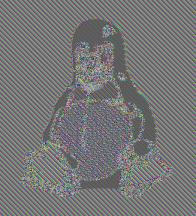
\includegraphics[width=0.3\textwidth]{imatges/Tux_ecb.jpg}}
  \subfloat[Algun dels modes segurs]{\label{fig:mode_sec}
\includegraphics[width=0.3\textwidth]{imatges/Tux_secure.jpg}}
  \caption{Exemple de com pot ser d'important el mode de xifrat el\lgem{}egit.}
  \label{fig:modes}
\end{figure}

Aquest sistema concatena el proc\'es de xifrar d'un bloc amb el seg\"uent de manera que s'afegeix dispersi\'o i augmenta la entropia a la xifra final. Tamb\'e extret de la \emph{Viquip\`edia} tenim en les figures \ref{fig:Cfb_encryption} i \ref{fig:Cfb_decryption} amb el diagrama de xifrat i el de desxifrat respectivament. En aquest mode el que es fa es xifrar un vector inicial que s'emmascara amb una operaci\'o \emph{xor} amb el text pla, per despr\'es reutilitzar la xifra com a seg\"uent entrada del pas seg\"uent. Per al desxifrat el procediment es molt similar, per\`o ara la xifra s'utilita per desemmascarar el valor de l'operaci\'o \emph{xor} i per realimentar els posteriors passos.

\begin{figure}[ht]
\centering
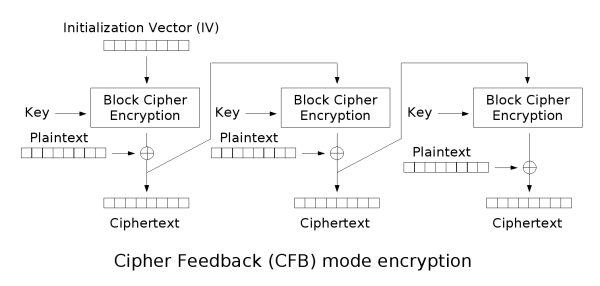
\includegraphics[width=1\textwidth]{imatges/Cfb_encryption.png}
\caption{Diagrama de xifrat de blocs amb el sistema CFB, extret de la \emph{Viquip\`edia}.\label{fig:Cfb_encryption}}
\end{figure}

\begin{figure}[ht]
\centering
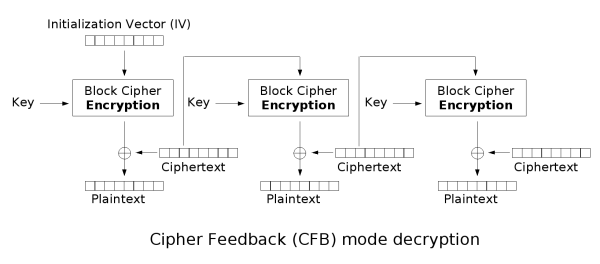
\includegraphics[width=1\textwidth]{imatges/Cfb_decryption.png}
\caption{Diagrama de desxifrat de blocs amb el sistema CFB, extret de la \emph{Viquip\`edia}.\label{fig:Cfb_decryption}}
\end{figure}

% \begin{itemize}
% \item \cite{BS96}
% \item \cite{MZ}
% \end{itemize}

\subsection{Protecci\'o: coordenades projectives \emph{vs} coordenades afins}\label{subsec:protecProject}

En primera inst\`ancia, l'\'us de coordenades projectives era una e\lgem{}ecci\'o matem\`atica, per\'o resulta una gran eina per protegir una implementaci\'o a atacs laterals passius com els descrits en \cite{KJJ}. Es tracta d'introduir soroll a un possible atacant que pugui estar escoltant l'electr\`onica amb que estem treballant.

Com s'ha explicat a la secci\'o \ref{sec:plans}, concretament amb la definici\'o \ref{def:coorproj}, un pla projectiu bidimensional \'es representa amb una terna de valors. Un punt d'un pla af\'{\i} \'es representat per una recta en un pla projectiu i tots els punts d'aquesta recta formen una classe d'equival\`encia que es la representaci\'o d'un sol punt. Recordem l'equaci\'o:
\begin{equation}\label{eq:project;ch:atacsLaterals}
\left( x,y,z\right) \sim \left( x\prime ,y\prime ,z\prime \right) \Rightarrow \exists \lambda \in \F^\star : x=\lambda x \prime, y=\lambda y \prime, z=\lambda z \prime
\end{equation}

Una operaci\'o de \emph{producte per un escalar} \'es realitza usant un algorisme molt eficient que recorre bit a bit l'escalar i realitza operacions \emph{suma de punts} i/o de \emph{duplicat d'un punt} segons si el bit del pas del bucle es un $0$ o un $1$. Aquestes dues operacions tenen costos diferents i per un atacant que n'analitzi el consum el\`ectric pot veure patrons de consum. El moment de realitzar l'operaci\'o es pot a\"{\i}llar i sobreposant algunes mostres es pot extreure informaci\'o de quin \'es el secret guardat sota un \ecdlp{} tipus $P=\left[d\right]G$ com l'enunciat en \ref{def:ecdlp}.

Com tenim una representaci\'o multiple d'un punt a trav\'es de qualsevol valor $\lambda$ aleatori amb el que emmascarem el punt, tot i que el valor del recorregut de bits sigui el mateix (l'escalar no ha variat), el nombre de mostres necess\`aries per un atac d'an\`alisi lineal augmenta.

En el cap\'{\i}tol \ref{ch:GnuPG} \'es descriu amb m\'es detall l'estat actual de la implementaci\'o d'aquesta protecci\'o.

%%%%%%%%%%%%%%%%%%%%%%%%%%%%%%%%%%%%%%%%%%%%%%%%%%%%%%%%%%%%%%%%%%%%%%%%%%%%%%%%%%%%%%%%%%%%%%%%%%%%%%%%%%%%
\subsection{La protecci\'o per isomorfismes del subgrup $\langle G\rangle$}\label{subsec:protecIsomorf}

Tot i que encara no em definit qu\`e \'es un isomorfisme, que \'es far\`a en la secci\'o \ref{subsec:isomorf}, concretament amb la definici\'o \ref{def:isomorf}. De moment, sols cal tenir present el seu significat sem\`antic dient que un isomorfisme d'un grup, \'es un altre grup diferent per\`o que mant\'e la mateixa ``forma''.

La protecci\'o indicada en \ref{subsec:protecProject} a n l'utilitzar coordenades projectives resulta \'util per donar un cert emmascarament, per\`o no fa variar el valor escalar secret amb el que s'opera. Es poden aprofitar isomorfismes de grups per variar el generador del \sgc{} que no aporten una protecci\'o matem\`atica a l'algorisme per\`o si a la firma e\lgem{}\`ectrica de les operacions. Aix\'i es pot canviar de generador
$$\left\langle G\right\rangle \equiv\left\langle G'\right\rangle \Longrightarrow\exists k\in\Fp^*\text{, tal que }G=[k]G'.$$
D'aquesta manera tenim una igualtat
$$P= \left[d\right]G = \left[d\right]\left[k\right]G',$$
que en permet protegir l'implementaci\'o del ECC d'avant d'an\`alisi diferencials de l'empremta el\`ectrica descrits en \cite{KJJ}.

Tamb\'e en aquest cas, aquesta protecci\'o ja te una implementaci\'o sobre el m\`odul escrit per la rama 1.4 del \emph{GnuPG}.

%% Potser faltaria entrar una mica més en detall, que aix'o sembla jo ho dic i ho heu de creure

% \begin{itemize}
% \item Escriptura equivalent de dos subgrups generadors $\left\langle G\right\rangle \equiv\left\langle G'\right\rangle \Leftrightarrow\exists k\subset\Fp |G=k\cdot G'$
% \item Similar a l'us de les coordenades projectives
% \item handicap de l'arrel quadrada modular
% \end{itemize}

%% TODO: no recordo d'on surt el Ecomentari de l'arrel quadrada modular. S'ha de repassar l'algorisme d'isomorfisme i probablement introduïr-lo aquí.

%%%%%%%%%%%%%%%%%%%%%%%%%%%%%%%%%%%%%%%%%%%%%%%%%%%%%%%%%%%%%%%%%%%%%%%%%%%%%%%%%%%%%%%%%%%%%%%%%%%%%%%%%%%%
\chapter{Reseteig d'un criptosistema: Estrelles d'isog\`enies}\label{ch:EstrellesIso}
%%%%%%%%%%%%%%%%%%%%%%%%%%%%%%%%%%%%%%%%%%%%%%%%%%%%%%%%%%%%%%%%%%%%%%%%%%%%%%%%%%%%%%%%%%%%%%%%%%%%%%%%%%%%

La criptografia de \ce{} presenta diverses avantatges respecte la criptografia sobre \cfs. La longitud del cos sobre el que es treballa pot ser molt menor, a dia d'avui podem confrontat una clau \emph{ElGamal} de $2048$ bits amb una clau el\lgem{}\'{\i}ptica de $224$ bits. Tot i que s'utilitzi una estructura de clau p\'ublica com la especificada en la norma \cite{ECPGP}, que pot fer que la clau rondi els $500$ bits, segueix essent molt menor. Tamb\'e presenta avantatges de c\`omput ja que les operacions per un usuari l\'{\i}cit tenen menys cost. Per\`o hi ha una avantatge molt major de les \ces{} que no s'aprofita: la seva facilitat a canviar de corba per resetejar el criptosistema i invalidar un atac.

Les dues primeres avantatges resulten molt bones per sistemes limitats. Ja sigui per la capacitat de comput, disponibilitat de mem\`oria o ample de banda, les \ces{} s\'on molt \'utils. Per\`o els est\`andards suggereixen l'us d'un nombre molt limitat de corbes, de manera que un atac sobre una pot afectar a totes les claus fetes amb ella. La soluci\'o d'elegir-ne una altra \ce{} major {\bf no} \'es bona per aquests sistemes m\'es limitats, ja que acostumen a estar molt dedicats a una longitud degut a la seva limitaci\'o. De tota manera, per als sistema que no sofreixen limitacions estrictes d'aquests tipus tampoc es bo ja que s'hi perd una gran agilitat.

Una soluci\'o passa per que en la generaci\'o del parell de claus \emph{p\'ublica-privada} sigui generada una \ce{} nova, aleat\`oria i que, molt important, compleixi una bona llista de requisits, com per exemple que s'evitin situacions susceptibles de ser atacades de les formes explicades com atacs dir\`ectes en la secci\'o \ref{sec:atacsDirectes}. Es una soluci\'o excessivament costosa per a l'usuari final.

Una segona aproximaci\'o passa per proporcionar una variabilitat major de corbes en cada longitud que, tot i limitar les longituds elegibles si aportaria diferents nivells de protecci\'o en base a les necessitats.

Per\`o, i si es pogues oferir que cada usuari, en el moment de generar el seu parell de claus, aconseguis una \ce{} pr\`opia amb un cost de producci\'o raonable? Aqu\'{\i} vam veure que les estrelles d'isog\`enies poden tenir joc. Cap la possibilitat que utilitzan un criptosistema basat en estrelles d'isog\`enies descrit en \cite{PkIso} un proposit diferent al inicialment plantejat pels autors, i \'es planteja aqu\'{\i} per al reseteig d'un criptosistema.

%%%%%%%%%%%%%%%%%%%%%%%%%%%%%%%%%%%%%%%%%%%%%%%%%%%%%%%%%%%%%%%%%%%%%%%%%%%%%%%%%%%%%%%%%%%%%%%%%%%%%%%%%%%%
\section{Isomorfismes i isog\`enies}
%%%%%%%%%%%%%%%%%%%%%%%%%%%%%%%%%%%%%%%%%%%%%%%%%%%%%%%%%%%%%%%%%%%%%%%%%%%%%%%%%%%%%%%%%%%%%%%%%%%%%%%%%%%%

Com passa amb la critografia amb \cf{} en front l'amena\c{c}a l'un criptoanalista canviar la clau secreta utilitzant la mateixa longitud del grup no invalida l'atac. Cal per aix\`o canviar de corba que sovint implica augmentar la longitud a una de m\'es bits. De ser aix\'{\i}, una gran virtud de les \ces{} \'es perd en no res.

Cal poder iniciar, i tamb\'e reiniciar, el ECC amb una \ce{} nova de manera que tot l'atac realitzat contra una corba no pugui ser portat a la nova que s'ha elegit. \cite{PkIso} i \cite{isoTFC} s\'on un article i un treball final de carrera on es planteja un criptosistema basat en estrelles d'isog\`enies. No coincideix amb el nostre prop\`osit ja que en el citat article els elements amb els que es descriu l'esquema criptogr\`afic s\'on les \ces{} dins d'una estructura d'anells on els nodes representen \ce{} i les arestes transicions d'isog\`enia.

En canvi el que busquem nosaltres \'es fer un recorregut per aquesta estructura d'anell per conseguir una nova \ce{} criptogr\`aficament \'util. Principalment que, per a un atacant, portar aquest criptoan\`alisi de la corba inicial a la nova sigui tant costos, i si pot ser m\'es, que tornar a comen\c{c}ar el criptoan\`alisi sobre el nou \sgc{}.

L'escull principal d'aquest algorisme de reseteig \'es el prop\`osit de ser molt m\'es eficient que crear una \ce{} criptogr\`aficament \'util des de zero. \'Es m\'es, la restricci\'o ha de ser que el temps de creaci\'o d'un parell de claus e\lgem{}\'{\i}ptiques ha de ser un temps raonable per a que un usuari ho reprodueixi en el seu computador; incl\'us en un de limitat com un empotrat o una targeta inte\lgem{}igent.

Hem estat dient que el ECC que es defineix ara \'es absolutament est\`atic. Tot el proc\'es de generar la tupla \ref{def:tupla} i el seus valors ens arriba recomanat pels valor indicats en l'ann\`ex \emph{E} de l'article \cite{NIST186}. Tamb\'e podem utilitzar altres \ces, com les proposades en \cite{brainpool} o les definides en \cite{sec2}. Per\'o totes tenen en com\'u que l'\'unic que difereix, al usar-les, entre dues claus \'es el valor privat \emph{d}; compartint la \ce{} tamb\'e es comparteix el criptoan\`alisi.

El reseteig de la \ce{} \'es un proc\'es que haur\`a de ser possible de realitzar tant a la generaci\'o est\`andard d'una clau com en qualsevol moment de la vida de la mateix. Amb claus sobre \cfs{} la validesa d'una clau sempre est\`a en funci\'o de la seva longitud i de tant en tant es modifica el valor de la caducitat. Amb \ce{} podem ser capa\c{c}os de generar una clau a l'inici que resulta diferent a la de la resta, i despr\'es d'un temps, on caducaria i la renovariem, procedir\'{\i}em a fer un reseteig, de manera que tindr\'{\i}em una nova corba amb una nova clau equivalent i tot criptoan\`alisi quedaria obsolet.

%%%%%%%%%%%%%%%%%%%%%%%%%%%%%%%%%%%%%%%%%%%%%%%%%%%%%%%%%%%%%%%%%%%%%%%%%%%%%%%%%%%%%%%%%%%%%%%%%%%%%%%%%%%%
\subsection{Qu\`e \'es un isomorfisme?}\label{subsec:isomorf}

Abans de definir una \emph{isog\`enia} i l'estructura proposada en \cite{PkIso} em de comen\c{c}ar per definir que \'es un isomorfisme. Un isomorfisme no aporta una major seguretat en front dels atacs directes als algorismes, per\'o hem vist que la seva utilitat amb els atacs laterals \ref{sec:atacsLaterals}.

En general si $\mathcal{A}$ i $\mathcal{B}$ son estructures algebr\`aiques del mateix tipus i $f:\;\mathcal{A}\rightarrow\mathcal{B}$ \'es una aplicaci\'o entre elles, es diu que $f$ \'es un \emph{morfisme} entre $\mathcal{A}$ i $\mathcal{B}$, quan l'aplicaci\'o ``respecta'' les operacions, es a dir, quan l'imatge per $f$ d'una operaci\'o en $\mathcal{A}$ \'es el mateix que operar en $\mathcal{B}$ les imatges dels operands. Si $\mathcal{A}=\mathcal{B}$ a $f$ se l'anomena un \emph{endomorfisme}. Quan $f$ \'es bijectiva, es parla d'\emph{isomorfisme}. Per concretar vegem qu\`e \'es un morfisme de grups. Siguin $(\mathcal{G},\circ)$ i $(\mathcal{G}',\ast)$ dos grups i  $f:\;\mathcal{G}\rightarrow\mathcal{G}'$ una aplicaci\'o entre ells. Direm que $f$ \'es un morfisme entre aquests dos grups quan per qualsevol element $a,b\in\mathcal{G}$ sigui $f(a\circ b)=f(a)\ast f(b)$. Formalment podem donar la definici\'o seg\"uent.
\begin{defi}\label{def:isomorf} Donats dos grups $(\mathcal{G},\circ)$ i $(\mathcal{G}',\ast)$ direm que son isomorfs si existeix una aplicaci\'o bijectiva $f$ entre $\mathcal{G}$ i $\mathcal{G}'$, tal que
$$\begin{array}{rcl}f:\;\mathcal{G} &\longrightarrow &\mathcal{G}',\\ f(a\circ b) &\longmapsto & f(a)\ast f(b),\end{array}$$
es a dir, $f$ \'es un morfisme bijectiu entre ambdos grups.
\end{defi}
Usarem m\'es endavant el concepte de \emph{n\'ucli} d'uns morfismes entre \ces{} anomenats \emph{isog\`enies}. Definim ara l'idea de n\'ucli d'un morfisme de grups.
\begin{defi}\label{def:ker} Si $\mathcal{G}\xrightarrow{f}\mathcal{G}'$ \'es un morfisme entre grups, el n\'ucli (o \emph{kernel}) d'aquest morfisme \'es el conjunt d'elements del primer grup $\mathcal{G}$ que s'apliquen en l'element neutre del segon $\mathcal{G}'$, es a dir,
$$\ker f=\{a\in\mathcal{G}:\;f(a)=e'\}\text{, essent $e'$ el neutre de }\mathcal{G}'.$$
\end{defi}
Es demostra f\`acilment que s\'{\i} $f$ \'es un morfisme de grups el seu n\'ucli $\ker f$ \'es un subgrup del primer d'ells,

En el cas del \sgc{} usat per definir el logaritme discret e\lgem{}\'{\i}ptic de la definici\'o \ref{def:ciclic}, tenim un punt $G\in E(\Fp)$ de $\mathrm{ord}(G)=n$ que genera aquest \sgc{} del grup de punts, $\langle G\rangle\subseteq E(\Fp)$. S\'{\i} $G'\in E(\Fp)$ \'es tamb\'e d'ordre $n$, \'es f\`acil veure que la seg\"uent aplicaci\'o entre $\langle G\rangle$ i $\langle G'\rangle$,
$$\begin{array}{rcl}f:\; \langle G\rangle &\longrightarrow &\langle G'\rangle,\\ f([k]G) &\longmapsto & [k]G',\forall k\in\{0,\dots,n-1\},\end{array}$$
\'es un isomorfisme de grups. En la pr\`actica, es mant\'e una corba precalculada com per exemple una del \cite{NIST186}, per la que $|E(\Fp)|=hn$, amb cofactor $h\lll n$ i $n$ primer (per aquestes corba NIST \'es $h=1$), i es pot generar el punt $G'$ com un punt aleatori en $E(\Fp)$ vigilant que {\bf no} tingui l'ordre del cofactor (definici\'o \ref{def:cofactor}), tindrem un isomorfisme, com l'explicat anteriorment, entre el \sgc{} recomanat $\langle G\rangle$ i el $\langle G'\rangle$.

%%%%%%%%%%%%%%%%%%%%%%%%%%%%%%%%%%%%%%%%%%%%%%%%%%%%%%%%%%%%%%%%%%%%%%%%%%%%%%%%%%%%%%%%%%%%%%%%%%%%%%%%%%%%
\subsection{Qu\`e \'es una isog\`enia?}\label{subsec:isogenia}

\begin{defi}\label{def:isogenia} Donades dos \ces{} $E/\K$ i $E'/\K$, son \emph{isog\`enes sobre $\K$} \textbf{sii} existeix una aplicaci\'on racional $E\xrightarrow{\mathcal{I}}E'$ que transforma $\mathcal{O}_{E}$ en $\mathcal{O}_{E'}$, es a dir,
\begin{equation}\label{eq:isogenia}\begin{array}{rcl}\mathcal{I}:\;E & \longrightarrow & E',\\ (x,y) & \longmapsto & (X,Y), \\ \mathcal{O}_{E} & \longmapsto  & \mathcal{O}_{E'},\end{array}\end{equation}
on $X$ i $Y$ responen a $X=f_{1}(x)$ i $Y=f_{2}(x,y)$, essent $f_{1}$ i $f_{2}$ funcions $\K$\/-racionals, i.e., quocients de polinomis de $\K[x,y]$. A l'aplicaci\'o $\mathcal{I}$ se l'anomena \emph{isog\`enia sobre $\K$} entre les \ces{} $E$ i $E'$.
\end{defi}

Les corbes is\'ogenies tenen un parell de propietats que ens interessen especialment i que enunciem breument.
\begin{enumerate}
	\item\label{isog:it1} S\'{\i} $\mathcal{I}: E/\Fp\rightarrow E'/\Fp$ \'es una isog\`enia, llavors $\mathcal{I}$ tamb\'e \'es un morfisme dels grups de punts, es a dir, per qualsevol parell $P,Q\in E(\Fp)$ es compleix que 
$$\underbrace{\mathcal{I}(P+Q)}_{\text{en }E(\Fp)}=\underbrace{\mathcal{I}(P)+\mathcal{I}(Q)}_{\text{en }E'(\Fp)}.$$
	\item\label{isog:it2} S\'{\i} $E/\Fp$ i $E'/\Fp$ s\'on is\`ogenes llavors tenen el mateix cardinal,
$$|E(\Fp)|=|E'(\Fp)|,$$ 
i rec\'{\i}procament, si dues \ces{} $E/\Fp$ i $E'/\Fp$ tenen el mateix cardinal llavors existeix una isog\`enia, sobre $\Fp$, entre elles.
\end{enumerate}

Les isog\`enies entre \ces{} definides sobre \cfs{} que nosaltres usarem permeten la seg\"uent definici\'o de \emph{grau de la isog\`enia}.
\begin{defi}[Grau d'una isog\`enia] Donada una isog\`enia $E/\Fp\xrightarrow{\mathcal{I}}E'/\Fp$ definirem el seu \emph{grau} com el cardinal del seu n\'ucli, $|\ker\mathcal{I}|$.\end{defi}
L'escenari en el que pensem que s\'on d'utilitat les isog\`enies entre \ces{} \'es el d'un ECC que es suposa en risc i que s'ha de \emph{resetejar}. Es pot reiniciar tot el ECC o es pot passar a una altra \ce{} is\`ogena amb l'inicial del ECC. Aquesta manera, segons l'apartat \ref{isog:it2} anterior, els par\`ametres del ECC associats al cardinal de la corba, l'ordre $n$ del grup criptogr\`afic, el cofactor $h$ i, clar, el propi cardinal $|E(\Fp)|$ no var\"{\i}en. Igualment es pot mantenir la clau s\'ecreta $1<d<n$, tot i que canviant la p\'ublica $P=[d]G$, al seu punt isogen, ja que per l'apartat \ref{isog:it1} es tindr\`a 
\begin{equation}\label{eq:isoclav}\mathcal{I}(P)=\mathcal{I}([d]G)=[d]\mathcal{I}(G).\end{equation}
Per\`o en un reseteig per canvi de corba a una is\'ogena, apareix un altre problema: s\'{\i} es coneix l'isog\`enia l'atacant del ECC pot aplicar-la als punts que hagi anat calculant en el seu atac i aix\'{\i} fer v\`alid aquest atac per la nova corba. El reseteig no haur\`a servit de res. \'Es, doncs, important que l'isog\`enia, concretament el seu grau, no sigui conegut per l'atacant. Per aix\'o poden servir les anomenades \emph{estrelles d'isog\`enies}.

Aix\'i com s'ha dit, i es veur\`a m\'es endavant que un \emph{isomorfisme} no es efectiu contra atacs directes, per\`o si ho es contra atacs laterals (\ref{sec:atacsLaterals}), una \emph{isog\`enia} {\bf si} resulta efectiva davant un atac directe contra el criptosistema descrit en la secci\'o \ref{sec:atacsDirectes}.

%%%%%%%%%%%%%%%%%%%%%%%%%%%%%%%%%%%%%%%%%%%%%%%%%%%%%%%%%%%%%%%%%%%%%%%%%%%%%%%%%%%%%%%%%%%%%%%%%%%%%%%%%%%%
\subsection{Volcans, serralades i estrelles de \ce}\label{subsec:volcans}

S'han comentat les cites \cite{PkIso} i \cite{isoTFC}, on es proposa utilitzar les \emph{isog\`enies} per resetejar un ECC, utilitzant estructures composades per \ces{} isog\`enas. El cam\'{\i} seguit per arribar a una \ce{} en aquestes estructures \'es un cam\'{\i} f\`acil de realitzar, per\`o computacionalment molt dur de resseguir per un atacant. Concretament, en el citat article \cite{PkIso} \'es considera el problema d'atacar una estructura de isog\`enies con un problema dur incl\'us per un hipot\`etic computador qu\`antic.

Les isog\`enies de \ce{} poden formar estructures i visualitzar-les en forma de grafs. Diferenciant les caracter\'{\i}stiques de com obtenir una transici\'o d'isog\`enia ens permeten constru\"{\i}r formes que ens recordin objectes del nostre imaginari. En diem volc\`a d'isog\`enies per la forma que li fem agafar a la vegada que a un conjunt de volcans en diem serralada. Exemple clar d'aix\`o tamb\' e son les estrelles d'isog\`enies.

\begin{defi}\label{def:volca} Definim un $\ell$-\emph{volc\`a} com un graf dirigit on els nodes son \ces{} i les arestes representen isog\`enies de grau $\ell$.\end{defi}
Aquests grafs --\/\emph{volcans} tenen una estructura ``per pisos'' porque cada corba--node pot tenir fins $\ell+1$ $\ell$\/-isog\`enies. Cada una d'elles t\'e una orientaci\'o, a saber, \emph{horitzontal}, \emph{descendent} o \emph{ascendent}, que es pot determinar a partir dels \emph{anells d'endomorfismes} de las corbas de partida i d'arribada. Degut a aquestes direccions possibles, podem constru\"{\i}r un graf que tindr\`a forma de volc\`a, format per un ciclo--\/\emph{cr\`ater}, on dels seus nodes o v\`ertex pengen arbres $\ell$-\/\`aris complets, excepte el cas que el volc\`a estigui redu\"{\i}t a sols el cr\`ater. Totes les fulles dels subarbres del volc\`a estan en el mateix nivell per a tot el volc\`a. Excepte les fulles, tots el nodes del volc\`a tenen $\ell+1$ arestes. Concretament, els nodes dels subarbres tenen una isog\`enia ascendent i $\ell$ descendents i les del cr\`ater en tenen dues d'horitzontals i $\ell-1$ descendents. Un exemple de vol\`a el podem veure en la figura \ref{fig:volca} que s'ha extret d'una figura de l'article \cite{VolcanIso}.

\begin{figure}[ht]
\centering
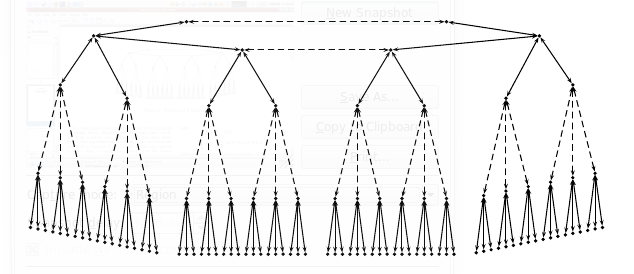
\includegraphics[width=0.8\textwidth]{imatges/volca.png}
\caption{Exemple de volc\`a extret de \cite{VolcanIso}.\label{fig:volca}}
\end{figure}

S\'{\i} aquests grafs constru\"{\i}ts mitjan\c{c}ant $\ell$\/-isog\`enies no son connexos, obtenim un conjunto de volcans que es poden denominar \emph{serralades}: totes les corbes--node de tots els volcans tindran, doncs, el mateix cardinal. Per\`o fixada una s\'olo son accessibles, per composici\'o repetida de $\ell$\/-isog\`enies, les que estan en el mateix volc\'a.

Considerem ara $\ell_i$\/-volcans d'isog\`enies per diferents primers $\ell_i$, tots ells redu\"{\i}ts al cr\'ater, i constru\"{\i}ts a partir de una mateixa corba $E/\Fp$. En aquest cas, els multiples camins de isog\`enies es veuen superposats i ordenats de manera que prenen formes de pol\'{\i}gons estrellats. D'aqu\'{\i} que a aquest graf se'l coneix com \emph{estrella d'isog\`enies}. En la figura~\ref{fig:estrella} en diferents colors estan representats els diferents cicles que s\'on cada $\ell_i$\/-cr\`ater.

\begin{figure}[ht]
\centering
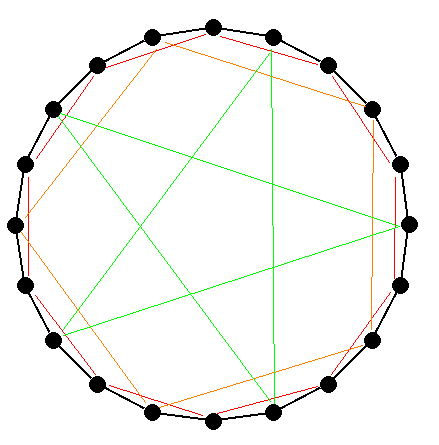
\includegraphics[width=0.5\textwidth]{imatges/estrella2.png}
\caption{Exemple d'estrella d'isog\`enies\label{fig:estrella}}
\end{figure}

%%%%%%%%%%%%%%%%%%%%%%%%%%%%%%%%%%%%%%%%%%%%%%%%%%%%%%%%%%%%%%%%%%%%%%%%%%%%%%%%%%%%%%%%%%%%%%%%%%%%%%%%%%%%
%%%%%%%%%%%%%%%%%%%%%%%%%%%%%%%%%%%%%%%%%%%%%%%%%%%%%%%%%%%%%%%%%%%%%%%%%%%%%%%%%%%%%%%%%%%%%%%%%%%%%%%%%%%%
\section{Possibilitats de l'\'us d'estrelles de \ces}

Al moment actual, les simulacions per tal d'obtenir una nova \ce{} a partir d'una inicial com\'u no han resultat satirfactories. Es tracta principalment que sigui un proc\'es que un usuari pugui realitzar i que prengui un temps raonable pel temps de generar una claus nou. Per corbes relativament petites els temps son considerables i desanimen a intentar-ho per corbes majors. La intenci\'o es aproximar el temps de creaci\'o d'un parell de claus e\lgem{}\'{\i}ptiques utilitzant isog\`enies, al temps de creaci\'o d'un parell de claus en \cfs{} d'un nivell de seguretat equivalent.

Hi ha un problema afegit a aquesta resticci\'o, i \'es que les corbes que recomanen els est\`andard no son les millors corbes per aplicar-hi algorismes d'isog\`enia i compliquen l'ideal de trobar un procediment que calculi una nova \ce{} criptogr\`aficament \'util en un temps raonable.

S'est\`a buscant que el sistema de \emph{setting} o \emph{resetting} de un parell de claus e\lgem{}\'{\i}ptiques sigui computable per part de l'usuari final. Es podrien precalcular desenes de corbes que despr\'es fossin seleccionades per d'usuari, per\`o l'obligariem a confiar en el nostre bon fer a l'hora d'\emph{``oblidar''} el cam\'{\i} recorregut per trobar la seva corba. En criptografia sempre ser\`a molt millor oferir un algorisme confiable i una bona implementaci\'o i que l'usuari pugui auditar tot el procediment. Aix\'{\i}, com es vol que el proc\'es l'executi l'usuari, ha de ser un proc\'es que requereixi d'un temps sensat per ser computat en les plataformes on corri el binaris finals.

Resulta primordial, doncs, que el temps de creaci\'o d'un parell de claus e\lgem{}\'{\i}ptiques noves sigui de l'ordre de la creaci\'o d'un parell de claus sobre \cfs{} d'una longitud equivalent segons la taula donada en la secci\'o 12 de \cite{ECPGP}. Actualment podem dir que estem molt lluny d'aquest objectiu ja que el sistema proposat en articles i treballs utilitzen \ces{} sobre uns \cfs{} minsos. Amb la implementaci\'o actual, la creaci\'o d'un parell de claus e\lgem{}\'{\i}ptiques resulta molt r\`apid doncs com a m\`axim es generar\`a una clau secreta $d$ d'una longitud d'uns $521$ bits; mentre la la creaci\'o d'una clau en \cfs{} de $2048$ bits requereix m\'es temps, consumeix molta m\'es entropia i sols \'es equivalent a una clau e\lgem{}\'{\i}ptica de $224$ bits.

L'us d'estrelles d'isog\`enies per (re)setejar el criptosistema no hauria de superar els temps sobre \cfs{} i aix\`o no sembla trivial d'aconseguir amb les simulacions realitzades fins ara. L'algorisme es senzill per\`o tenim que conseguir que els seus passos es puguin realitzar molt de presa.

\begin{table}[H]
\begin{algo}[Procediment de Setting d'una \ce{}]\label{alg:isogenia}
 \parbox[b]{\linewidth}{%
\hrule
\smallskip
{\bf INPUT:}: Primer $p$ sobre el que definir la \ce{} \EFpbis{} i $k$ longitud del recorregut a realitzar.

{\bf OUTPUT}: Una \ce{} sobre un \cf{}, d'una estrella d'isog\`enies.
\vspace{1.5mm}
\hrule
}%
\begin{algorithmic}[1]
\STATE Seleccionar una \ce{} inicial $E_{0}$ sobre \Fp;
\STATE Generar una ruta aleat\`oria $L$ de longitud $k$ d'elements \\ $L=\left\{r_{0},r_{1},\dots,r_{k}\right\},t.q. \forall r\in_{R}...$;%!! d'on son aquests elements
\STATE $E' \leftarrow L\left(E_{0}\right)$; \\ /*Calcular la corba $E'$ resultant del recorregut $L$ en l'estrella  */
\STATE Retornar $E'$;
\end{algorithmic}
\end{algo}
\end{table}

% comentar que una ruta es una llista ordenada d'elements de ...
Es un algorisme similar a un de xifrat, per\`o del que podem i devem oblidar els valors aleat\`oria de la llista per tal de mantenir aquest viatge per dins l'estrella en secret. Si ni tant sols es guarda, segur que no podr\`a deixar-se exposat. El proc\'es de reseteig no seria molt diferent ja que tampoc resulta recomanable mantenir la clau secreta antiga podent escollir un valor nou de clau secreta $d$ per obtenir una clau p\'ublica en la nova \ce{}.

%%%%%%%%%%%%%%%%%%%%%%%%%%%%%%%%%%%%%%%%%%%%%%%%%%%%%%%%%%%%%%%%%%%%%%%%%%%%%%%%%%%%%%%%%%%%%%%%%%%%%%%%%%%%
\chapter{Gnu Privacy Guard}\label{ch:GnuPG}
%%%%%%%%%%%%%%%%%%%%%%%%%%%%%%%%%%%%%%%%%%%%%%%%%%%%%%%%%%%%%%%%%%%%%%%%%%%%%%%%%%%%%%%%%%%%%%%%%%%%%%%%%%%%

Quan el projecte \cite{BM04} va comen\c{c}ar no existien grans pretencions, per\`o si la i\lgem{}usi\'o de veure'l integrat en el \emph{GnuPG}. Es important fer software lliure, per\`o no s'ha de deixar que la feina realitzada quedi en l'oblit i es perdi.

%%%%%%%%%%%%%%%%%%%%%%%%%%%%%%%%%%%%%%%%%%%%%%%%%%%%%%%%%%%%%%%%%%%%%%%%%%%%%%%%%%%%%%%%%%%%%%%%%%%%%%%%%%%%
\section{Assignment - GNU GPG}\label{sec:assigGnu}
%%%%%%%%%%%%%%%%%%%%%%%%%%%%%%%%%%%%%%%%%%%%%%%%%%%%%%%%%%%%%%%%%%%%%%%%%%%%%%%%%%%%%%%%%%%%%%%%%%%%%%%%%%%%

Despr\'es de un llarg treball que culminar amb l'implementaci\'o d'un pegat per la rama \emph{1.4} del programa lliure \emph{GnuPG} es va iniciar un projecte de manteniment i millora amb la publicaci\'o d'una petita p\`agina web on allotjar els fonts del projecte i la seva documentaci\'o de cara a l'escrutini p\'ublic.

Va funcionar. Poc m\'es de 6 mesos despr\'es, sobre el novembre de 2004, un company rus, de nom Mikael Mylnikov, es va posar en contacte per indicar un mal funcionament o bug en l'implementaci\'o de la signatura digital. La implementaci\'o era capa\c{c} de verificar signatures que no eren. Era una errada greu que havia passat per alt als tests realitzats i uns bons ulls extern van poder veure. La trobada de l'error significa l'inici d'un bon treball que culmina amb l'aportaci\'o d'un algorisme de xifrat m\'es robust. La publicaci\'o com a program\`ari lliure ha pres un sentit complert.

Molt posteriorment es va iniciar un \emph{fil de discusi\'o}\footnote{El podem trobar a l'adre\c{c}a http://lists.gnupg.org/pipermail/gnupg-devel/2007-March/023725.html} en la llista de desenvolupadors del \emph{GnuPG} on es demanava suport per \ce{} en la llibreria \emph{libgcrypt}. El codi del projecte \cite{BM04} va ser portat per en \emph{Werner Koch} del pegat preparat per la rama $1.4$ cap a la mencionada llibreria matem\`atica i criptogr\`afica de la branca $2$ (en aquell moment branca $1.9$) del \emph{GnuPG}.

%Despr\'es d'un fil en la llista de desenvolupament en la llista del \emph{GnuPG} el mar\c{c} de 2007, Werner koch porta la fima digital del pegat per la rama \emph{1.4} del \emph{GnuPG} a la llibreria matem\`atica \emph{libgcrypt} que es el m\`odul encarregat dels algoritmes per a la rama \emph{2} (\emph{1.9} en aquell moment) del mateix \emph{GnuPG}.

El fet de tenir ja la signatura digital portada anima a implicar-se amb aquest programa i a proposar l'aportaci\'o m\'es directa i din\`amica de codi. Aix\`o t\'e dues opcions: agreements puntuals amb la \emph{Free Software Fundation} i el projecte \emph{GNU} per tal d'aportar algunes l\'{\i}nies o arribar a un acord i signar un assignment amb la \emph{FSF} i formar part dels desenvolupadors i mantenedors d'aquest software. A partir d'aquesta signatura, s'entra a formar part del grup de desenvolupadors que poden enviar codi per la seva avaluaci\'o i posterior publicaci\'o.

% \section{GNU coding standard}
% 
% (...)

\section{Dos branques, dos codis}\label{sec:branques}

S'ha comentat a la secci\'o \ref{sec:assigGnu} l'aparici\'o en la llibreria matem\`atica \emph{libgcrypt} de suport per a \ce{} escrit per en \emph{Werner Koch} basat en el pegat \cite{BM04}. Despr\'es s'ha comentat l'entrada al grup de desenvolupadors del \emph{GnuPG}. I tot aix\`o junt porta a l'actual manteniment de dues branques de codi: una (amb unes primitives) per al \emph{GnuPG} 1.4.x, i una altra per a la \emph{libgcrypt} 1.4.y (usat pel \emph{GnuPG} 2.0.z).

\'Es important veure clar com es fan les coses en cada programa de cara a mantenir una sola l\'{\i}nia sense diverg\`encies ni de disseny ni d'implementaci\'o i a la vegada esfor\c{c}ar-se a no cometre errors. Amb tota probabilitat, el desenvolupament es centrar\`a en el treball en la llibreria deixant obsolet el pegat del projecte \cite{BM04}. Actualment s'est\`a treballant per implementar l'est\`andard \cite{ECPGP} que s'ha comentat en la secci\'o \ref{subsec:ECPGP} i els algorismes s'han comentat en la secci\'o \ref{subsec:eccopenpgpalg}.

A continuaci\'o es presenten unes taules on es divideixen en blocs les funcions, m\`etodes i primitives de les dues implementacions publicades; contraposant-les i oferint una visi\'o del que cadascuna implementa i com ho defineix. No s'han incl\`os aquelles funcions que estan essent incloses per\`o que no apareixen actualment en els repositoris p\'ublics. Indicar tamb\'e que s'ha seguit per a definici\'o aqu\'{\i} el \emph{coding standard} del projecte \emph{Gnu}.

La primera de les taules \'es fonamental. A la taula \ref{tab:struct} recopila les estructures de dades implementades per les dues branques en el referent a l'implementaci\'o de \ce{}. Resulta fonamental pel fet que ser\`a continuament referenciada des de que es vulgui passar un parametre o refer\`encia a qualsevol de les funciones de la resta de taules. Entre les dues branques no hi ha difer\`encies m\'es que en la nomenclatura de les variables, el contingut de l'estructura segueix sent el mateix. Hi ha per\`o si algunes estructures noves en la \emph{libgcrypt} i aix\`o es deu a una millor implementaci\'o de l'assignaci\'o de valor preestablerts en els est\`andards i normatives comentats en la secci\'o \ref{subsec:normes}.

La taula \ref{tab:interface} recull d'Interf\'{\i}cie entre el n\'ucli en les diferents rames i el m\`odul propiament. El \emph{GnuPG} resulta exemplar en aplicar be patrons i el que fa es tractar cada algorisme o criptosistema com una unitat. D'aqu\'{\i} va venir que el projecte \cite{BM04} estiques completament codificat en un fitxer de codi i un de cap\c{c}alera. Com veurem en posteriors taules, la llibreria \emph{libgcrypt} dona un pas m\'es i trasllada el codi m\'es matem\`atic cap a l'interior del seu nucli de c\`alcul criptogr\`afic.

Destacar que algunes funcions d'Interf\'{\i}cie primordials, com son el xifrat i el desxifrat no tenen contrapartida en la columna de la \emph{libgcrpt}, aix\`o es deu a que aquesta llibreria sols t\'e publicada en aquest moment l'algorisme \emph{ECDSA} i que s'ampliar\`a en breu cap al suport de l'est\`andard \cite{ECPGP} que s'ha esmentat en la secci\'o \ref{subsec:ECPGP}.

Succeeix el mateix per parlar de la taula \ref{tab:cryptGeneral} on les funcions de xifrat i desxifrat no mostren especificaci\'o en la segona columna i es per la mateixa ra\'o, ja que sols s'estan mostran aquelles funcions que es poden descarregar des del repositori p\'ublic. Si, per\`o, queda patent la refer\`encia feta a la traducci\'o directa d'estructures (taula \ref{tab:struct}) ja que tant la firma com la verificaci\'o l'esquema seguit es el mateix.

%\ref{tab:cryptAux}
Entrant amb m\'es detall cap a l'interior del m\`etodes criptogr\`afics tenim la taula \ref{tab:cryptAux} amb els m\`etodes que no son cridats directament per l'Interf\'{\i}cie citada en la taula \ref{tab:interface}. Principalment son els m\`etodes que defineixen la generaci\'o d'un parell de claus i tot el seu setup. Per exemple, l'us de estrelles d'isog\`enies del que s'ha parlat en el cap\'{\i}tol \ref{ch:EstrellesIso} modificaria el contingut de la funci\'o {\tt generate\_curve()} i no afectaria a la resta que ja han estat pensats per no dependre de una llista est\`atica de corbes.

Queden tamb\'e en aquesta taula \ref{tab:cryptAux} uns m\`etodes al final que tenen relaci\'o directa amb el sistema de xifrat proposat en \cite{BM06}. L'implementaci\'o del xifrat en la \emph{libgcrypt} est\`a feta seguint el proposat a \cite{ECPGP} llavors els m\`etodes criptogr\`afics auxiliars seran uns altres i es veur\`a que la traducci\'o no \'es possible. Els algorismes son incompatibles entre ells de manera que es descarta la seva conviv\`encia.

%\ref{tab:math}
La taula \ref{tab:math} presenta forats a totes dues bandes i es deu a diferents motius. Els primers m\`etodes que sols existeixen, de moment en el pegat per la rama 1.4 del \emph{GnuPG} es deuen a que en aquest s'implementa la protecci\'o al atacs laterals de la secci\'o \ref{subsec:protecIsomorf} per utilitzar un isomorfisme del grup generador aix\'{\i} com tamb\'e l'us de diferents representacions projectives d'un punt com es deia en la secci\'o \ref{subsec:protecProject}.

Tamb\'e estan en la taula que tractem ara i estan en les dues rames les funcions fonamentals per les operacions de suma de punts que es deien en les definicions \ref{def:sumaEracional}, duplicat d'un punt de la definici\'o \ref{def:duplEracional} i la fonamental per al logaritme discret e\lgem{}\'{\i}ptic que es la {\tt escalarMult()} que prov\'e de la definici\'o \ref{def:multEracional}.

Al final d'aquesta taula \ref{tab:math} es fan refer\`encia a m\'etodes per operar enters del \cf{} base sobre el que viu la \ce{}. Aix\`o es deu a que l'efic\`acia dels m\`etodes gen\`erics de la llibreria \emph{libgcrypt} no resulten eficients per als proporcionalment mes curts valors de les coordenades d'un punt de \ce{}.

%\ref{tab:useStrucs}
Finalment ja sols ens queda una taula, la \ref{tab:useStrucs} que tanca el cicle al ser l'\'ultim nivell que a m\'es enlla\c{c}a amb la primera taula \ref{tab:struct}, la de les estructures, i aqu\'{\i} hi ha els m\`etodes sobre com inicialitzar o alliberar la mem\`oria d'aquestes, copiar-les, o resoldre l'equaci\'o de la \ce{}.

\lstset{language=C,basicstyle=\footnotesize,breaklines=true}
% \begin{sideways}
% \begin{tabular}{|l|l|l|l|}
% \hline
% Patch 1.4 & \multicolumn{3}{c|}{libgcrypt} \\
% \hline
%  {\sf cipher/ecc.c}     & {\sf cipher/ecc.c} & {\sf mpi/ec.c} & {\sf src/mpi.h} \\



\begin{table}[H]
\begin{center}
\begin{sideways}
\begin{tabular}{|l||l|l|}
\hline
Patch 1.4 & \multicolumn{2}{c|}{libgcrypt} \\
\hline
 {\sf cipher/ecc.c}     & {\sf cipher/ecc.c} & {\sf src/mpi.h} \\

\hline
 {\tt \begin{lstlisting}{}
typedef struct{
  MPI x_;
  MPI y_;
  MPI z_;
} point; 
 \end{lstlisting} }
 &&
 {\tt \begin{lstlisting}{}
struct mpi_point_s;
typedef struct mpi_point_s mpi_point_t;
struct mpi_point_s {
  gcrypt_mpi_t x;
  gcrypt_mpi_t y;
  gcrypt_mpi_t z;
};
 \end{lstlisting} }\\
\hline
 {\tt \begin{lstlisting}{}
typedef struct {
  MPI p_;
  MPI a_,b_;
  point G;
  MPI n;
} ellipticCurve;
 \end{lstlisting} }
 &
 {\tt \begin{lstlisting}{}
typedef struct {
  gcrypt_mpi_t p;
  gcrypt_mpi_t a,b;
  mpi_point_t G;
  gcrypt_mpi_t n;
} elliptic_curve_t;
 \end{lstlisting} }
 &\\
\hline
 {\tt \begin{lstlisting}{}
typedef struct {
  ellipticCurve E;
  point Q;
} ECC_public_key;
 \end{lstlisting} }
 &
 {\tt \begin{lstlisting}{}
typedef struct {
  elliptic_curve_t E;
  mpi_point_t Q;
} ECC_public_key;
 \end{lstlisting} }
 &\\
\hline
 {\tt \begin{lstlisting}{}
typedef struct {
  ellipticCurve E;
  point Q;
  MPI d;
} ECC_secret_key;
 \end{lstlisting} }
 &
 {\tt \begin{lstlisting}{}
typedef struct {
  elliptic_curve_t E;
  mpi_point_t Q;
  gcrypt_mpi_t d;
} ECC_secret_key;
 \end{lstlisting} }
 &\\
\hline
 &
 {\tt \begin{lstlisting}{}
static const struct {
  const char *name;
  const char *other;
} curve_aliases[]
 \end{lstlisting} }
 &\\
\hline
 &
 {\tt \begin{lstlisting}{}
static const struct {
  const char *desc;
  unsigned int nbits;
  const char *p;
  const char *a,*b;
  const char *n;
  const char *g_x,*g_y;
} domain_params[]
 \end{lstlisting} }
 &\\
\hline
 &
 {\tt \begin{lstlisting}{}
static const char *ecdsa_names[]
 \end{lstlisting} }
 &\\
\hline
 &
 {\tt \begin{lstlisting}{}
gcry_pk_spec_t
_gcry_pubkey_spec_ecdsa
 \end{lstlisting} }
 &\\
\hline
\end{tabular}
\end{sideways}
\end{center}
\caption{Taula d'estructures utilitzades en les rames del \emph{GnuPG}\label{tab:struct}}
\end{table}


\begin{table}
\begin{center}
%\begin{sideways}
\begin{tabular}{|l|l|}
\hline
Patch 1.4 & libgcrypt \\
\hline
 {\sf cipher/ecc.c}     & {\sf cipher/ecc.c} \\
\hline
{\tt \begin{lstlisting}{}
int
ecc_generate(int algo,
    unsigned nbits,
    MPI *skey,
    MPI **refactors)
\end{lstlisting} }
&
{\tt \begin{lstlisting}{}
gcry_err_code_t
_gcry_ecc_generate(int algo,
      unsigned int nbits,
      const char *curve,
      gcry_mpi_t *skey,
      gcry_mpi_t **retfactors)
static gcry_err_code_t
ecc_generate(int algo,
    unsigned int nbits,
    unsigned long dummy,
    gcrypt_mpi_t *skey,
    gcry_mpi_t **retfactors)
\end{lstlisting} }
\\
\hline
{\tt \begin{lstlisting}{}
int
ecc_check_secret_key(int algo,
    MPI *skey)
\end{lstlisting} }
&
{\tt \begin{lstlisting}{}
static gcry_err_code_t
ecc_check_secret_key(int algo, 
    gcry_mpi_t *skey)
\end{lstlisting} }
\\
\hline
{\tt \begin{lstlisting}{}
int
ecc_encrypt(int algo, MPI *resarr,
    MPI data, MPI *pkey)
\end{lstlisting}}
&\\
\hline
{\tt \begin{lstlisting}{}
int
ecc_decrypt(int algo, MPI *result,
    MPI *data, MPI *skey)
\end{lstlisting} }
&\\
\hline
{\tt \begin{lstlisting}{}
int
ecc_sign(int algo, MPI *resarr,
    MPI data, MPI *skey)
\end{lstlisting} }
&
{\tt \begin{lstlisting}{}
static gcry_err_code_t
ecc_sign(int algo,
    gcry_mpi_t *resarr,
    gcry_mpi_t data,
    gcry_mpi_t *skey)
\end{lstlisting} }
\\
\hline
{\tt \begin{lstlisting}{}
int
ecc_verify(int algo, MPI hash,
    MPI *data, MPI *pkey)
\end{lstlisting} }
&
{\tt \begin{lstlisting}{}
static gcry_err_code_t
ecc_verify(int algo, gcry_mpi_t hash,
    gcry_mpi_t *data,
    gcry_mpi_t *pkey,
    int (*cmp)(void *,gcry_mpi_t),
    void *opaquev)
\end{lstlisting} }
\\
\hline
{\tt \begin{lstlisting}{}
unsigned int
ecc_get_nbits(int algo, MPI *pkey)
\end{lstlisting} }
&
{\tt \begin{lstlisting}{}
static unsigned int
ecc_get_nbits(int algo,
    gcry_mpi_t *pkey)
\end{lstlisting} }
\\
\hline
{\tt \begin{lstlisting}{}
const char *
ecc_get_info(int algo, int *npkey,
    int *nskey, int *nenc,
    int *nsig, int *use)
\end{lstlisting} }
&\\
\hline
&
{\tt \begin{lstlisting}{}
gcry_err_code_t
_gcry_ecc_get_param(const char *name,
      gcry_mpi_t *pkey)
\end{lstlisting} }
\\
\hline
&
{\tt \begin{lstlisting}{}
static gcry_mpi_t
ec2os(gcry_mpi_t x, gcry_mpi_t y,
      gcry_mpi_t p)
\end{lstlisting} }
\\
\hline
&
{\tt \begin{lstlisting}{}
static gcry_error_t
os2ec(mpi_point_t *result,
      gcry_mpi_t value)
\end{lstlisting} }
\\
\hline

\end{tabular}
%\end{sideways}
\end{center}
\caption{Taula amb les funcions d'interficie d'un m\`odul del \emph{GnuPG}\label{tab:interface}}
\end{table}

\begin{table}
\begin{center}
\begin{tabular}{|l|l|}
\hline
Patch 1.4 & libgcrypt \\
\hline
 {\sf cipher/ecc.c}     & {\sf cipher/ecc.c} \\
\hline
 {\tt \begin{lstlisting}{}
static void
doEncrypt(MPI input, 
          ECC_public_key *pkey, 
          point *R, MPI c)
      \end{lstlisting} }
 & \\
\hline
 {\tt \begin{lstlisting}{}
static MPI
decrypt(MPI output,
        ECC_secret_key *skey,
        point *R, MPI c)
      \end{lstlisting} }
 & \\
\hline
 {\tt \begin{lstlisting}{}
static void
sign(MPI input,
     ECC_secret_key *skey,
     MPI *r, MPI *s)
      \end{lstlisting} }
 &
 {\tt \begin{lstlisting}{}
static gpg_err_code_t
sign(gcry_mpi_t input,
     ECC_secret_key *skey,
     gcry_mpi_t r, gcry_mpi_t s)
      \end{lstlisting} } \\
\hline
 {\tt \begin{lstlisting}{}
static int
verify(MPI input,
       ECC_public_key *pkey,
       MPI r, MPI s)
      \end{lstlisting} }
 &
 {\tt \begin{lstlisting}{}
static gpg_error_code_t
verify(gcry_mpi_t input,
       ECC_public_key *pkey,
       gcry_mpi_t r, gcry_mpi_t s)
      \end{lstlisting} } \\
\hline
\end{tabular}
\end{center}
\caption{Taula amb els m\`etodes criptogr\`afics generals \label{tab:cryptGeneral}}
\end{table}

\begin{table}
\begin{center}
\begin{sideways}
\begin{tabular}{|l|l|}
\hline
Patch 1.4 & libgcrypt \\
\hline
 {\sf cipher/ecc.c}     & {\sf cipher/ecc.c} \\
\hline
 {\tt \begin{lstlisting}{}
static MPI
gen_k(MPI p, int secure)
      \end{lstlisting} }
 &
 {\tt \begin{lstlisting}{}
static gcry_mpi_t
gen_k(gcry_mpi_t p,
      int security_level)
      \end{lstlisting} }
 \\
\hline
 {\tt \begin{lstlisting}{}
static void
generateCurve(unsigned nbits,
     ellipticCurve *ECC_curve)
      \end{lstlisting} }
 &
 {\tt \begin{lstlisting}{}
static gpg_err_code_t
generate_curve(unsigned int nbits,
            const char *name,
            elliptic_curve_t *curve,
            unsigned int *r_nbits)
      \end{lstlisting} }
 \\
\hline
 {\tt \begin{lstlisting}{}
static void
generateKey(ECC_secret_key *sk, 
            unsigned nbits)
      \end{lstlisting} }
 &
 {\tt \begin{lstlisting}{}
static gpg_err_code_t
generate_key(ECC_secret_key *sk,
             unsigned int nbits,
             const char *name,
             gcry_mpi_t g_x, gcry_mpi_t g_y,
             gcry_mpi_t q_x, gcry_mpi_t q_y)
      \end{lstlisting} }
 \\
\hline
 {\tt \begin{lstlisting}{}
static void
testKeys(ECC_secret_key *sk,
         unsigned nbits)
      \end{lstlisting} }
 &
 {\tt \begin{lstlisting}{}
static void
test_keys(ECC_secret_key *sk,
          unsigned int nbits)
      \end{lstlisting} }
 \\
\hline
 {\tt \begin{lstlisting}{}
static int
check_secret_key(ECC_secret_key *sk)
      \end{lstlisting} }
 &
 {\tt \begin{lstlisting}{}
static int
check_secret_key(ECC_secret_key *sk)
      \end{lstlisting} }
 \\
\hline
 {\tt \begin{lstlisting}{}
static void
progress(int c)
      \end{lstlisting} }
 &
 {\tt \begin{lstlisting}{}
void
_gcry_register_pk_ecc_progress(void (*cb)
    (void *, const char *, int, int, int),
    void *cb_data)
      \end{lstlisting} }
 \\
\hline
 {\tt \begin{lstlisting}{}
static void
sha256_hashing(MPI input,
             MPI *output)
      \end{lstlisting} }
 & \\
\hline
 {\tt \begin{lstlisting}{}
static void
aes256_encrypting(MPI key, MPI input,
              MPI *output)
      \end{lstlisting} }
 & \\
\hline
 {\tt \begin{lstlisting}{}
static void
aes256_decrypting(MPI key, MPI input,
                MPI *output)
      \end{lstlisting} }
 & \\
\hline
\end{tabular}
\end{sideways}
\end{center}
\caption{Taula amb m\`etode criptogr\`afics auxiliars \label{tab:cryptAux}}
\end{table}

\begin{table}
\begin{center}
\begin{tabular}{|l|l|}
\hline
Patch 1.4 & libgcrypt \\
\hline
 {\sf cipher/ecc.c}     & {\sf mpi/ec.c} \\
\hline
 {\tt \begin{lstlisting}{}
static int
genBigPoint(MPI prime,
       ellipticCurve *base,
       point *G,
       unsigned nbits)
      \end{lstlisting} }
 & \\
\hline
 {\tt \begin{lstlisting}{}
static point
genPoint(MPI prime,
  ellipticCurve *base)
      \end{lstlisting} }
 & \\
\hline
 {\tt \begin{lstlisting}{}
static MPI
modularSquareRoot(MPI a,
            MPI modulus)
      \end{lstlisting} }
 & \\
\hline
 {\tt \begin{lstlisting}{}
static MPI
symbolLegendre(MPI n,
          MPI modulus)
      \end{lstlisting} }
 & \\
\hline
 {\tt \begin{lstlisting}{}
static int
PointAtInfinity(point Query)
      \end{lstlisting} }
 & \\
\hline
 {\tt \begin{lstlisting}{}
static void
escalarMult(MPI escalar,
     point *P, point *R,
     ellipticCurve *base)
      \end{lstlisting} }
 &
 {\tt \begin{lstlisting}{}
void
_gcry_mpi_ec_mul_point(mpi_point_t *result,
                       gcry_mpi_t scalar,
                       mpi_point_t *point,
                       mpi_ec_t ctx)
      \end{lstlisting} }
 \\
\hline
 {\tt \begin{lstlisting}{}
static void
sumPoints(point *P0,
   point *P1,
   point *P2,
   ellipticCurve *base)
      \end{lstlisting} }
 &
 {\tt \begin{lstlisting}{}
void
_gcry_mpi_ec_add_points(mpi_point_t *result,
           mpi_point_t *p1, mpi_point_t *p2,
           mpi_ec_t ctx)
      \end{lstlisting} }
 \\
\hline
 {\tt \begin{lstlisting}{}
static void
duplicatePoint(point *P,
     point *R,
     ellipticCurve *base)
      \end{lstlisting} }
 &
 {\tt \begin{lstlisting}{}
void
_gcry_mpi_ec_dub_point(mpi_point_t *result,
          mpi_point_t *point, mpi_ec_t ctx)
      \end{lstlisting} }
 \\
\hline
 {\tt \begin{lstlisting}{}
static void
invertPoint(point *P,
  ellipticCurve *base)
      \end{lstlisting} }
 & \\
\hline
 &
 {\tt \begin{lstlisting}{}
static void
ec_addm(gcry_mpi_t w, gcry_mpi_t u,
        gcry_mpi_t v, mpi_ec_t ctx)
      \end{lstlisting} }
 \\
\hline
 &
 {\tt \begin{lstlisting}{}
static void
ec_subm(gcrt_mpi_t w, gcry_mpi_t u,
        gcry_mpi_t v, mpi_ec_t ctx)
      \end{lstlisting} }
 \\
\hline
 &
 {\tt \begin{lstlisting}{}
static void
ec_mulm(gcrt_mpi_t w, gcry_mpi_t u,
        gcry_mpi_t v, mpi_ec_t ctx)
      \end{lstlisting} }
 \\
\hline
 &
 {\tt \begin{lstlisting}{}
static void
ec_powm(gcrt_mpi_t w, const gcry_mpi_t b,
        const gcry_mpi_t e, mpi_ec_t ctx)
      \end{lstlisting} }
 \\
\hline
 &
 {\tt \begin{lstlisting}{}
static void
ec_invm(gcrt_mpi_t x,
        gcry_mpi_t a,
        mpi_ec_t ctx)
      \end{lstlisting} }
 \\
\hline
\end{tabular}
\end{center}
 \caption{Taula amb les funcions matem\`atiques\label{tab:math}}
\end{table}

\begin{table}
 \begin{center}
\begin{sideways}
\begin{tabular}{|l||l|l|}
\hline
Patch 1.4 & \multicolumn{2}{c|}{libgcrypt} \\
\hline
 {\sf cipher/ecc.c}     & {\sf cipher/ecc.c} & {\sf src/mpi.h} \\
\hline
 {\tt \begin{lstlisting}{}
static point
point_copy(point *P)
      \end{lstlisting} }
 &
 {\tt \begin{lstlisting}{}
static void
point_set(mpi_point_t *d,
          mpi_point_t *s)
      \end{lstlisting} }
 &
 {\tt \begin{lstlisting}{}
static void
point_set(mpi_point_t *d,
          mpi_point_t *s)
      \end{lstlisting} }
 \\
\hline
 &
 {\tt \begin{lstlisting}{}
#define point_init(a)
_gcry_mpi_ec_point_init((a))
      \end{lstlisting} }
 &
 {\tt \begin{lstlisting}{}
#define point_init(a)
_gcry_mpi_ec_point_init((a))
void
_gcry_mpi_ec_point_init(mpi_point_t *p)
      \end{lstlisting} }
 \\
\hline
 {\tt \begin{lstlisting}{}
static void
point_free(point P)
      \end{lstlisting} }
 &
 {\tt \begin{lstlisting}{}
#define point_free(a)
_gcry_mpi_ec_point_free((a))
      \end{lstlisting} }
 &
 {\tt \begin{lstlisting}{}
#define point_free(a)
_gcry_mpi_ec_point_free((a))
void
_gcry_mpi_ec_point_free(mpi_point_t *p)
      \end{lstlisting} }
 \\
\hline
 {\tt \begin{lstlisting}{}
static int
point_affine(point P, MPI x,
  MPI y, ellipticCurve *base)
      \end{lstlisting} }
 & &
 {\tt \begin{lstlisting}{}
int
_gcry_mpi_ec_get_affine(gcry_mpi_t x,
    gcry_mpi_t y, mpi_point_t *point,
    mpi_ec_t ctx)
      \end{lstlisting} }
 \\
\hline
 & &
 {\tt \begin{lstlisting}{}
mpi_ec_t
_gcry_mpi_ec_init(gcry_mpi_t p,
                  gcry_mpi_t a)
      \end{lstlisting} }
 \\
\hline
 {\tt \begin{lstlisting}{}
static ellipticCurve
curve_copy(ellipticCurve *E)
      \end{lstlisting} }
 &
 {\tt \begin{lstlisting}{}
static elliptic_curve_t
curve_copy(elliptic_curve_t E)
      \end{lstlisting} }
 & \\
\hline
 {\tt \begin{lstlisting}{}
static void
curve_free(ellipticCurve E)
      \end{lstlisting} }
 &
 {\tt \begin{lstlisting}{}
static void
curve_free(elliptic_curve_t *E)
      \end{lstlisting} }
 &
 {\tt \begin{lstlisting}{}
void
_gcry_mpi_ec_free(mpi_ec_t ctx)
      \end{lstlisting} }
 \\
\hline
 {\tt \begin{lstlisting}{}
static MPI
get_bit()
      \end{lstlisting} }
 & & \\
\hline
 {\tt \begin{lstlisting}{}
static MPI
gen_y_2(MPI x,
    ellipticCurve *base)
      \end{lstlisting} }
 &
 {\tt \begin{lstlisting}{}
static gcry_mpi_t
gen_y_2(gcry_mpi_t x,
    elliptic_curve_t *base)
      \end{lstlisting} }
 & \\
\hline
 &
 {\tt \begin{lstlisting}{}
static gcry_mpi_t
scanval(const char *string)
      \end{lstlisting} }
 & \\
\hline
\end{tabular}
\end{sideways}
\end{center}
\caption{Taula amb m\`etodes per manupular estructures.\label{tab:useStrucs}}
\end{table}

%%%%% Estic repetint lo de la secció del assignment!!!
%El projecte de l'enginyeria t\`ecnica \cite{BM04} es va escriure en forma de pegat per la branca $1.4$ del \emph{GnuPG}. Amb els anys aquest pegat va anar evolucionant, corregint errors i ampliant-se. La seva vida en aquesta branca toca a la seva fi ja que el 20 de mar\c{c} de 2007 es va obrir un fil en la llista de desenvolupadors\footnote{http://lists.gnupg.org/pipermail/gnupg-devel/2007-March/023725.html} del GnuPG on es demanava suport per a \ces{} en la llibreria \emph{libgcrypt}. 


\chapter{Conclusions i treball futur}

% (...)
% \begin{enumerate}
%  \item implementaci\'o d'isog\`enies
%  \item implementaci\'o en la libgcrypt de l'openPGP
%  \item migrar el pegat per la branca 1.4 cap a la branca 2 del GnuPG. Utilitzant la libgcrypt tant pel xifrat com per la firma.
% \end{enumerate}

Recopilant la feina feta en aquest projecte queda desenvolupament pendent. El desenvolupament m\'es extens que queda \'es l'implementaci\'o de les isog\`enies. Com s'ha comentat \'es vol tenir unes restriccions per a la creaci\'o del parell de clau que, actualment, no resulten trivials d'assolir. La longitud del viatge dins de l'estrella d'isog\`enies feta amb una $\ell$-erralada definida en \ref{def:serralada} que t\'e la forma de la figura \ref{fig:estrella}.

A m\'es d'una trava matem\`atica a resoldre per una implementaci\'o r\`apida i eficient, hi ha una restricci\'o des dels est\`andards. L'est\`andard per a la implementaci\'o \cite{ECPGP}, que actualment est\`a en fase \emph{internet draft} per\`o que esdevindr\`a definitiu aviat, sols contempla una redu\"{\i}da de \ces{}, una per a cada longitud, codificant-la amb un index contingut en la clau. D'aquesta manera la clau resulta molt menor, per\`o dificulta usar-ne d'altres. En comunicaci\'o amb \emph{Andrey Jivson}, autor de l'est\`andard, la soluci\'o passaria per escriure un \emph{extension draft} per permetre altres t\'{\i}pus de corba i que aquestes puguin ser contingudes en la estructura de la clau.

En la branca 1.4 hi ha tenim les primitives necess\`aries per quasi totes les operacions que els c\`alculs de l'isog\`enia requereix per\`o un cop completat el recull de primitives aquestes existents haurien de ser revisades per a que el seu procediment sigui \`optim i no alenteixi el proc\`es de la mateixa manera que en la secci\'o \ref{sec:branques} s'ha vist que que les operacions sobre \cfs{} s'han d'optimitzar per la menor longitud i major repetibilitat amb que ens trobem quan usem \ces{}.

De tota manera el desenvolupament sobre la branca 1.4 toca a la seva fi, i el treball natural s'anir\`a decantant cap a directament la llibreria \emph{libgcrypt} i la branca 2 del \emph{GnuPG}. Per tant la ben pr\`oxima publicaci\'o de l'implementaci\'o de l'est\`andard \cite{ECPGP}, en especial l'apartat del xifrat i desxifrat, est\`a previst de fer-se ja solsament sobre l'implementaci\'o de la \emph{libgcrypt}, ampliant aix\'{\i} el suport que ja t\'e per l'algorisme de firma digital ECDSA.

Resumint, primordialment s'acabar\`a amb l'implementaci\'o del xifrat de \ce{} per a la rama 2, deixant-la a la mateixa posici\'o que la rama 1.4 (tot i que amb algorismes diferents) i deixant aquesta \'ultima en des\'us. Despr\'es es refor\c{c}ar\`a les implementacions, sota la cobertura dels est\`andards, proteccions als atacs laterals tractats en el cap\'{\i}tol \ref{ch:atacsLaterals} i en para\lgem{}el es vol posar en pr\`actica la viabilitat de les estrelles d'isog\`enies del cap\'{\i}tol \ref{ch:EstrellesIso}. Es preveu la publicaci\'o d'articles per part dels autors a cada pas que es vagi donant.


\begin{thebibliography}{1}
\vspace{5mm}
\bibitem{1} {\large\bf Llibres i revistes}
\bibitem[HANDECC]{HANDECC} Henri Cohen, Gerhard Frey \textit{Handbook of Elliptic and Hyperelliptic Curve Cryptography} Ed. Chapman \& Hall
\bibitem[LMS265]{LMS265} Ian Blake, Gadiel Seroussi, Nigel Smart, \textit{Elliptic Curve in Cryptography} Ed. Cambridge University Press
\bibitem[LMS317]{LMS317} Ian Blake, Gadiel Seroussi, Nigel Smart, \textit{Advances in Elliptic Curve Cryptography} Ed. Cambridge University Press
\bibitem[ECDSA]{JMV}D. Johnson, A. Menezes, S. Vanstone, \textit{The elliptic Curve Digital Signature Algorithm (ECDSA)}. Dept. of Combinatorics \& Optimization, University of Waterloo, Certicom, Canada.
\bibitem[Men93]{Men93}Alfred Menezes, \textit{Elliptic Curve Public Key Cryptosystems}. Kluwer Academic Publishers, 1993
\bibitem[BS96]{BS96} Bruce Schneier, \textit{Appiled cryptography}.
\bibitem[H9DL]{H9DL} Dineal Lerch, \emph{Criptograf\'{\i}a de Curva El\'{\i}ptica: Ataque de Rho de Pollard}, article en \emph{Hakin9}, hakin9.org/upload/hakin9/PDFVersion/curvas\_elipticas.pdf

\vspace{5mm}
\bibitem{2} {\large\bf Collita pr\`opia}
\bibitem[BM04]{BM04} Sergi Blanch, Ramiro Moreno, \emph{GnuPG Implementation with Elliptic Curves} Treball final de carrera, Enginyeria t\`ecnica en Inform\`atica de Sistemes, Universitat de Lleida. Mar\c{c} 2004.
\bibitem[BM04-1]{BM04-1} Sergi Blanch, Ramiro Moreno, \emph{Implementaci\'o GnuPG con Curvas El\'{\i}pticas} Recsi'04, Universidad Carlos III, 2004.
\bibitem[BM06]{BM06} Sergi Blanch, Ramiro Moreno, \emph{An\'alisis del cifrado ElGamal de un m\'odulo con curvas el\'{\i}pticas propuesto para el GnuPG} Recsi06, Universitat Aut\'onoma de Barcelona i Universitat Oberta de Catalunya, 2006.

\vspace{5mm}
\bibitem{3} {\large\bf Est\`andards}
\bibitem[P1363]{P1363}IEEE P1363/D13 (Draft Version 13) Standard Specifications for Public key Cryptography. 1999 November 12.
\bibitem[NIST197]{NIST197} FIPS PUB 197, Advanced Encryption Standard (AES), U.S.Department of Commerce/National Institute of Standards and Technology. 2001.
\bibitem[NIST180]{NIST180}FIPS PUB 180-2, Secure Hash Standard (SHS), U.S.Department of Commerce/National Institute of Standards and Technology. 2002.
\bibitem[NIST186]{NIST186}FIPS PUB 186-3, Digital Signature Standard (DSS), U.S.Department of Commerce/National Institute of Standards and Technology. March 2006.
\bibitem[NIST800]{NIST800} Nist Special Publication 800-56A \emph{Recommendation for Pair-Wise Key Establishment Schemes Using Discrete Logarithm Cryptography} March 2007.
\bibitem[ECPGP]{ECPGP} A. Jivsov, \textit{ECC in OpenPGP}, IETF internet Draft, April 2008
\bibitem[GNUSTD]{GNUSTD} R. Stallman, \textit{Gnu Coding Standards}, July 2005.
\bibitem[rfc2119]{2119} S. Bradner, \textit{Key words for use in RFCs to Indicate Requirement Levels}. 1997 March.
\bibitem[rfc3278]{3278} S. Blake-Wilson, D. Brown, P. Lambert, \textit{Use of Elliptic Curve Cryptography (ECC) Algorithms in Cryptographic Message Syntax (CMS)}. 2002 April.
\bibitem[rfc3394]{3394} J. Schaad, R. Housley, \textit{ Advanced Encryption Standard (AES) Key Wrap Algorithm} September 2002.
\bibitem[rfc4492]{4492} S. Blake-Wilson, N. Bolyard, V. Gupta, C. Hawk, B. Moeller, \textit{Elliptic Curve Cryptography (ECC) Cipher Suites for Transport Layer Security (TLS)}. 2006 May.
\bibitem[rfc4880]{4880} J. Callas, L. Donnerhacke, H. Finney, D. Shaw, R. Thayer, \textit{OpenPGP Message Format}. 2007 November
\bibitem[brainpool]{brainpool} ECC Brainpool Standard Curves and Curve Generation. 2005 October 19.
\bibitem[sec1]{sec1} SEC 1. Standards for Efficient Cryptography Group: Elliptic Curve Cryptography.
\bibitem[sec2]{sec2} SEC 2. Standards for Efficient Cryptography Group: Recommended Elliptic Curve Domain Parameters.

\vspace{5mm}
\bibitem{3} {\large\bf Atacs directes}
\bibitem[Silv99]{Silv99}J. Silverman, \textit{The Xedni calculus and the elliptic curve discrete logarithm problem}, Designs, codes and Cyptography, n20 (2000), 5-40.
\bibitem[Xedni99]{Xedni99}M. j. jacobson, N. Koblitz, J. H. Silverman, A. Stein, E. Teske, \textit{Analysis of the Xedni Calculus Attack}, 1999.

\bibitem[mov97]{handbook} Alfred J, Menezes, Paul C.van Oorschot, and Scott A. Vanstone. \textit{Handbook of Applied Cryptography}. CRC Press, first edition, 1997. http://cacr.math.uwaterloo.ca/hac/

\vspace{5mm}
\bibitem{4} {\large\bf Atacs laterals}
%side channel attacks
\bibitem[HAGAI]{HAGAI} Hagai Bar-El, \textit{Introduction to Side Channel Attacks} White paper, Discretix Technologies Ltd.
\bibitem[KJJ]{KJJ} Paul Kocher, Joshua Jaffe, Benjamin Jun, \textit{Introduction to Differential Power Analysis and Related Attacks} Cryptography Resarch Inc, San Fancisco.
\bibitem[BJN]{BJN} Dan Boneh, Antonie Joux and Phong Q. Nguyen, \textit{Why textbook ElGamal and RSA encryption are Insecure}.
\bibitem[MZ]{MZ} Serge Mister and Robert Zuccherato, \textit{An Attack on CFB Mode Encryption As Used By OpenPGP}

\vspace{5mm}
\bibitem{5} {\large\bf Isog\`enies}
\bibitem[MSTTV07]{VolcanIso} J, Miret, D. Sadornil, J. Tena, R. Tom\`as, M. Valls, \textit{Isogeny cordillera algorithm to obtain cryptographically good elliptic curves}.
\bibitem[MMSTV06]{comp2iso} J. Miret, R. Moreno, D. Sadornil, J. Tena, M. Valls, \textit{An algorithm to compute volcanoes of 2-isogenies of elliptic curves over finite fields}.
\bibitem[Galbr98]{ConstrIso} S. Galbraith, \textit{Constructing isogenies between elliptic curves over finite fields}.
\bibitem[LM98]{AlgoIso} R. Lercier, F. Morain, \textit{Algorithms for computing isogenies between elliptic curves}.
\bibitem[FM05]{AlgoSEA} M. Fouquet, F. Morain, \textit{Isogeny volcanoes and the SEA algorithm}.
\bibitem[BMSS06]{FastAlgoIso} A. Bostan, F. Morain, B. Salvy, E. Schost, \textit{Fast algorithms for computing isogenies between elliptic curves}.
\bibitem[RS06]{PkIso} A. Rostovtsev, A. Stolbunov, \textit{Public-key cryptosystem based on isogenies}.
\bibitem[MTRVM]{ParaIso} S. Martinez, R. Tom\`as, C. Roig, M. Valls, R. Moreno, \textit{Parallel Calculation of Volcanoes for Cryptographyc Uses}.
\bibitem[isoTFC]{isoTFC} R. Arias, J. Miret, \textit{Implementac\'on de un criptosistema de clave p\'ublica basado en estrellas de isogenias} TFC Ingenier\'{\i}a Inform\'atica UdL.

\end{thebibliography}

\end{document}
